% "THE BEER-WARE LICENSE" (Revision 42)
%
% Nicolas Iooss wrote this file in 2015.  As long as you retain this notice you
% can do whatever you want with this stuff. If we meet some day, and you think
% this stuff is worth it, you can buy me a beer in return.
\documentclass[a4paper,10pt]{article}
\usepackage[utf8]{inputenc}
\usepackage[T1]{fontenc}
\usepackage[francais]{babel}
\usepackage[pdftex]{hyperref}
\usepackage{geometry}
\usepackage{bbm}
\usepackage{color}
\usepackage{amsmath}
\usepackage{hyperref}
\usepackage{verbatim}
\usepackage{graphicx}
\usepackage[toc,page]{appendix}
\usepackage{xcolor}
\usepackage{pdfpages}

\geometry{%
a4paper,
body={160mm,250mm},
left=25mm,top=25mm,
headheight=7mm,headsep=4mm,
marginparsep=4mm,marginparwidth=5mm}

\hypersetup{
    colorlinks,
    linkcolor={blue!50!black},
    citecolor={blue!50!black},
    urlcolor={blue!80!black}
}

% SciTE coloration
\setlength{\fboxsep}{0pt}
\newcommand{\scitea}[1]{\noindent{\ttfamily{\textcolor[rgb]{0.5, 0.5, 0.5}{\colorbox[rgb]{1.0, 1.0, 1.0}{#1}}}}}
\newcommand{\sciteb}[1]{\noindent{\ttfamily{\textcolor[rgb]{0.0, 0.5, 0.0}{\colorbox[rgb]{1.0, 1.0, 1.0}{#1}}}}}
\newcommand{\scitec}[1]{\noindent{\ttfamily{\textcolor[rgb]{0.0, 0.5, 0.5}{\colorbox[rgb]{1.0, 1.0, 1.0}{#1}}}}}
\newcommand{\scited}[1]{\noindent{\ttfamily{\textcolor[rgb]{0.5, 0.0, 0.5}{\colorbox[rgb]{1.0, 1.0, 1.0}{#1}}}}}
\newcommand{\scitee}[1]{\noindent{\ttfamily{\textcolor[rgb]{0.5, 0.0, 0.5}{\colorbox[rgb]{1.0, 1.0, 1.0}{#1}}}}}
\newcommand{\scitef}[1]{\noindent{\ttfamily{\textbf{\textcolor[rgb]{0.0, 0.0, 0.5}{\colorbox[rgb]{1.0, 1.0, 1.0}{#1}}}}}}
\newcommand{\sciteg}[1]{\noindent{\ttfamily{\textcolor[rgb]{0.5, 0.0, 0.5}{\colorbox[rgb]{1.0, 1.0, 1.0}{#1}}}}}
\newcommand{\sciteh}[1]{\noindent{\ttfamily{\textcolor[rgb]{0.5, 0.0, 0.0}{\colorbox[rgb]{1.0, 1.0, 1.0}{#1}}}}}
\newcommand{\scitei}[1]{\noindent{\ttfamily{\textbf{\textcolor[rgb]{0.0, 0.0, 1.0}{\colorbox[rgb]{1.0, 1.0, 1.0}{#1}}}}}}
\newcommand{\scitej}[1]{\noindent{\ttfamily{\textbf{\textcolor[rgb]{0.0, 0.5, 0.5}{\colorbox[rgb]{1.0, 1.0, 1.0}{#1}}}}}}
\newcommand{\scitek}[1]{\noindent{\ttfamily{\textbf{\textcolor[rgb]{0.0, 0.0, 0.0}{\colorbox[rgb]{1.0, 1.0, 1.0}{#1}}}}}}
\newcommand{\scitel}[1]{\noindent{\ttfamily{\textcolor[rgb]{0.0, 0.0, 0.0}{\colorbox[rgb]{1.0, 1.0, 1.0}{#1}}}}}
\newcommand{\scitep}[1]{\noindent{\ttfamily{\textcolor[rgb]{0.5, 0.3, 0.0}{\colorbox[rgb]{1.0, 1.0, 1.0}{#1}}}}}
\newcommand{\sciteib}[1]{\noindent{\ttfamily{\textcolor[rgb]{0.0, 0.0, 0.0}{\colorbox[rgb]{1.0, 1.0, 1.0}{#1}}}}}
\newcommand{\sciteqb}[1]{\noindent{\ttfamily{\textcolor[rgb]{0.5, 0.5, 0.0}{\colorbox[rgb]{1.0, 1.0, 1.0}{#1}}}}}
\newcommand{\sciterb}[1]{\noindent{\ttfamily{\textbf{\textcolor[rgb]{0.0, 0.0, 0.0}{\colorbox[rgb]{1.0, 1.0, 1.0}{#1}}}}}}
\newcommand{\scitevb}[1]{\noindent{\ttfamily{\textcolor[rgb]{0.0, 0.5, 0.5}{\colorbox[rgb]{1.0, 1.0, 1.0}{#1}}}}}
\newcommand{\scitewb}[1]{\noindent{\ttfamily{\textcolor[rgb]{0.0, 0.0, 0.0}{\colorbox[rgb]{1.0, 1.0, 1.0}{#1}}}}}
\newcommand{\scitexb}[1]{\noindent{\ttfamily{\textbf{\textcolor[rgb]{0.0, 0.0, 0.5}{\colorbox[rgb]{1.0, 1.0, 1.0}{#1}}}}}}
\newcommand{\sciteac}[1]{\noindent{\ttfamily{\textcolor[rgb]{0.5, 0.0, 0.5}{\colorbox[rgb]{1.0, 1.0, 1.0}{#1}}}}}
\newcommand{\scitebc}[1]{\noindent{\ttfamily{\textcolor[rgb]{0.5, 0.0, 0.5}{\colorbox[rgb]{1.0, 1.0, 1.0}{#1}}}}}
\newcommand{\scitecc}[1]{\noindent{\ttfamily{\textbf{\textcolor[rgb]{0.0, 0.0, 0.0}{\colorbox[rgb]{1.0, 1.0, 1.0}{#1}}}}}}

% Header
\title{Solution du challenge SSTIC 2015}
\author{Nicolas Iooss}
\date{\today}

\makeatletter
  \hypersetup{
    pdftitle = {\@title},
    pdfauthor = {\@author}
  }
\makeatother

% Custom commands
\newcommand{\todo}[1]{\fcolorbox{red}{yellow}{TODO: #1}}
\newcommand{\bksl}{\char`\\} % Backslash
\newcommand{\lsl}[1]{\textless{}\textless{} #1} % <<
\newcommand{\lsr}[1]{\textgreater{}\textgreater{} #1} % >>

\newcommand{\pyinput}[1]{%
    \noindent{\color[rgb]{0.5, 0.5, 0.5}{\rule{\textwidth}{0.4pt}}}
    \input{#1} \\
    \noindent{\color[rgb]{0.5, 0.5, 0.5}{\rule{\textwidth}{0.4pt}}}
}

\renewcommand{\appendixname}{Annexes}
\renewcommand{\appendixpagename}{Annexes}
\renewcommand{\appendixtocname}{Annexes}

% Document
\begin{document}
\maketitle

\section*{Résumé}

Cette année le challenge consistait à étudier l'image d'une carte microSD pour y trouver une adresse e-mail en @challenge.sstic.org.
Cette carte microSD contient un fichier pour Rubber Ducky qui permet, une fois connecté à un ordinateur, d'exécuter des commandes qui créent une archive zip.

Cette archive contient un fichier chiffré dont la clé de déchiffrement a été écrite sous forme d'énigme dans une carte OpenArena.

Une fois cette énigme résolue, il est possible de déchiffrer le fichier chiffré, qui est une autre archive zip contenant un second fichier chiffré dont il faut récupérer la clé de chiffrement qui a été ``enregistrée avec Paint''.
Après avoir compris ce que ceci signifie et trouvé la clé, le déchiffrement du fichier permet d'obtenir encore une fois une archive zip, mais qui contient cette fois ci une page HTML.

Cette page HTML contient un code Javascript obfusqué qui tente de déchiffrer un bloc de données en utilisant des paramètres de déchiffrement (vecteur d'initialisation et clé) issus de l'agent utilisateur du navigateur.

Une fois ces paramètres devinés, la cinquième étape du challenge consiste à comprendre le fonctionnement d'un réseau de transputers afin de casser l'algorithme de déchiffrement qui est implémenté sur celui-ci.

Le résultat de ce déchiffrement est une archive contenant une image au format JPEG de laquelle il faut extraire successivement des images aux formats PNG, TIFF et GIF qui sont cachées les unes dans les autres.
Finalement la dernière image extraite contient l'adresse e-mail qu'il faut trouver, permettant ainsi de valider la fin du challenge.

\clearpage
\tableofcontents

\setcounter{section}{-1} % Begin at section 0

\clearpage
\section{Premier avril}

Contrairement à ce qui a été annoncé dans le résumé, cette année le challenge du SSTIC n'a pas commencé directement par l'analyse de l'image d'une carte microSD mais par une annonce sur le compte Twitter du symposium le premier avril:

\begin{figure}[h!]
  \centering
  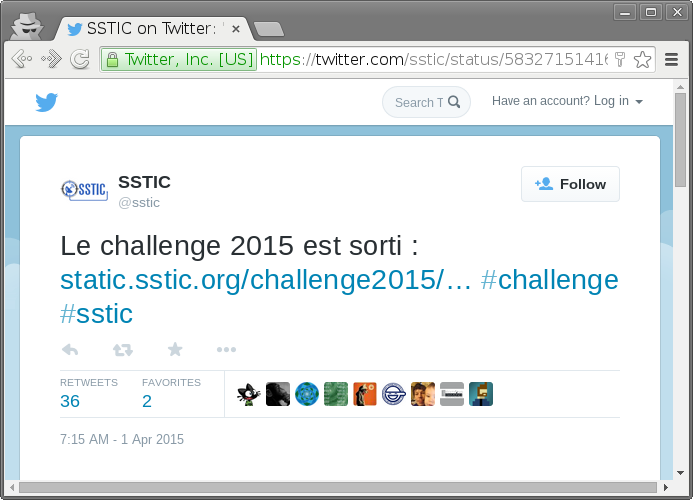
\includegraphics[width=10cm]{stage0/twitter-screenshot.png}
  \caption{\url{https://twitter.com/sstic/status/583271514163814400}}
\end{figure}

Ce tweet invite à télécharger \url{http://static.sstic.org/challenge2015/chlg-2015}.
Une rapide analyse de ce fichier binaire permet de trouver quelques informations intéressantes:

\begin{verbatim}
% binwalk chlg-2015
DECIMAL       HEXADECIMAL     DESCRIPTION
--------------------------------------------------------------------------------
0             0x0             OpenSSL encryption, salted, salt: 0x441980B6425FD4FF

% xxd chlg-2015 | head -8
00000000: 5361 6c74 6564 5f5f 4419 80b6 425f d4ff  Salted__D...B_..
00000010: 1e5c 83a1 c4d7 24f5 4697 9aac 2571 5f8e  .\....$.F...%q_.
00000020: 64e2 52ad 8947 119e c4ad 929b 6505 4de2  d.R..G......e.M.
00000030: ff44 0add d438 273c 4b8d 760d 416d c883  .D...8'<K.v.Am..
00000040: 290e 8014 1ce7 88a2 b6c7 cd00 d8e9 98bd  )...............
00000050: e40c cb76 4b52 626e 0ee0 c966 b1c8 c24b  ...vKRbn...f...K
00000060: e40c cb76 4b52 626e 0ee0 c966 b1c8 c24b  ...vKRbn...f...K
00000070: 4915 cd03 153c 5210 abe7 c68f c882 f198  I....<R.........
\end{verbatim}

Ce fichier commence par ``Salted\_\_'', qui correspond à l'entête d'un fichier chiffré par la commande openssl.
Le mot de passe utilisé pour chiffrer le fichier a été salé par le sel donné dans l'entête, mais ni ce mot de passe ni l'algorithme utilisé ne sont connus.

Néanmoins on remarque la répétition de la séquence \texttt{e40c cb76 4b52 626e 0ee0 c966 b1c8 c24b} aux positions hexadécimales 50 et 60.
Il est donc pertinent de chercher des séquences de 16 octets qui seraient beaucoup répétées dans le fichier:

\begin{verbatim}
% xxd -c16 -p chlg-2015 | sort | uniq -c | sort -n -k1 | tail
    210 0b7c95d5a80232a053290ea06d2fb0cf
    225 00a7342de61ab4b16a4683278e01e34f
    239 3d06a766ef80a06a053b80221b2c3d73
    242 3b7257deb0bd655d54e6a19621f5fccf
    244 f43238a9941a0df61eef2b5407f0f75c
    292 ea12dfa3e6261e8f2a80a84bda0caada
    326 96eadc039da237294066f0eed246e26c
    347 ff6757e5b67d8fbdf67d886987ec2512
   3563 e40ccb764b52626e0ee0c966b1c8c24b
 145511 ad07b6efc462dffead318a9501a14390
\end{verbatim}

Ainsi, le fichier a été chiffré par un algorithme qui a produit 3563 fois la séquence \texttt{e40c cb76 4b52 626e 0ee0 c966 b1c8 c24b} et 145511 fois \texttt{ad07 b6ef c462 dffe ad31 8a95 01a1 4390}.
Il s'agit donc probablement d'un algorithme de chiffrement par bloc qui utilise le mode Electronic CodeBook (ECB)\footnote{\url{https://en.wikipedia.org/wiki/Block_cipher_mode_of_operation\#ECB}}.
En tentant les algorithmes supportés par openssl qui utilisent le mode ECB (dont la liste dans dans la documentation \footnote{\url{https://www.openssl.org/docs/apps/enc.html\#SUPPORTED-CIPHERS}}) et en devinant quel mot de passe peut être utilisé, on trouve que le fichier a été chiffré par AES-128 en mode ECB avec le mot de passe \texttt{SSTIC}:

\begin{verbatim}
% openssl enc -d -aes-128-ecb -in chlg-2015 -out decrypted -k sstic
% file decrypted
decrypted: PC bitmap, Windows 95/NT4 and newer format, 1000 x 1000 x 24
\end{verbatim}

Le fichier déchiffré est donc une image bitmap, que voici.

\begin{figure}[h]
  \centering
  
\includegraphics[width=12cm]{stage0/pngsolution.png}
  \caption{Image déchiffrée}
\end{figure}

Malheureusement l'adresse e-mail n'a pas pour domaine @challenge.sstic.org.
Ce premier petit challenge est donc un poisson d'avril qui permet toutefois d'avoir un avant-goût du véritable challenge, au cours duquel il faut également déchiffrer des fichiers en trouvant des astuces.

\clearpage
\section{Un Rubber Ducky qui parle en PowerShell}

\subsection{De la carte microSD au script Rubber Ducky}

Le vrai challenge commence sur \url{http://communaute.sstic.org/ChallengeSSTIC2015}, par le téléchargement d'un fichier qui contient le contenu d'une ``carte microSD qui était insérée dans une clé USB étrange''.

L'archive zip du challenge\footnote{\url{http://static.sstic.org/challenge2015/challenge.zip}} contient un seul fichier, nommé \texttt{sdcard.img}.
Il s'agit probablement d'une copie brute du contenu de la carte microSD qu'il est demandé d'analyser. La commande \texttt{file} permet de déterminer qu'il s'agit d'un système de fichier FAT:
\begin{verbatim}
% file sdcard.img
sdcard.img: DOS/MBR boot sector, code offset 0x3c+2, OEM-ID "mkfs.fat",
sectors/cluster 4, root entries 512, Media descriptor 0xf8, sectors/FAT 244,
sectors/track 32, heads 64, sectors 250000 (volumes > 32 MB) , serial number
0xe50d883b, unlabeled, FAT (16 bit)
\end{verbatim}

Ce système de fichier ne contient qu'un seul fichier, nommé \texttt{inject.bin}, qui ne contient pas de texte.
Par ailleurs, l'exécution de \texttt{strings} sur \texttt{sdcard.img} révèle un contenu intéressant:
\begin{verbatim}
% strings -tx -5 sdcard.img | tail -3
  3d221 UILD   SH
  3d260 INJECT  BIN
  41a00 java -jar encoder.jar -i /tmp/duckyscript.txt
\end{verbatim}

En observant les octets aux alentours de ces chaînes de caractères on comprend mieux leur contexte:
\begin{verbatim}
% xxd -a sdcard.img | grep '^0003d'
0003d200: e562 0075 0069 006c 0064 000f 00bd 2e00  .b.u.i.l.d......
0003d210: 7300 6800 0000 ffff ffff 0000 ffff ffff  s.h.............
0003d220: e555 494c 4420 2020 5348 2020 0000 2d1e  .UILD   SH  ..-.
0003d230: 7a46 7a46 0000 2d1e 7a46 0300 2d00 0000  zFzF..-.zF..-...
0003d240: 4169 006e 006a 0065 0063 000f 00e4 7400  Ai.n.j.e.c....t.
0003d250: 2e00 6200 6900 6e00 0000 0000 ffff ffff  ..b.i.n.........
0003d260: 494e 4a45 4354 2020 4249 4e20 0000 3a1e  INJECT  BIN ..:.
0003d270: 7a46 7a46 0000 3a1e 7a46 0400 a2ab 0a02  zFzF..:.zF......
0003d280: 0000 0000 0000 0000 0000 0000 0000 0000  ................

% xxd -a sdcard.img | grep '^00041'
00041a00: 6a61 7661 202d 6a61 7220 656e 636f 6465  java -jar encode
00041a10: 722e 6a61 7220 2d69 202f 746d 702f 6475  r.jar -i /tmp/du
00041a20: 636b 7973 6372 6970 742e 7478 7400 0000  ckyscript.txt...
00041a30: 0000 0000 0000 0000 0000 0000 0000 0000  ................
\end{verbatim}

Le contenu à la position 3d200 ressemble fortement à une table de dossier qui contient deux entrées:
\begin{itemize}
  \item la première (de 3d200 à 3d23f) correspond à un fichier supprimé qui s'appelait \texttt{build.sh},
  \item et la seconde (de 3d240 à 3d27f) correspond au fichier \texttt{inject.bin} qui a déjà été trouvé.
\end{itemize}

Le texte à la position 41a00 correspondrait alors au contenu du fichier supprimé.

En résumé, la carte SD qui était insérée dans une clé USB étrange contient un fichier \texttt{inject.bin} de format non trivial et un fichier supprimé \texttt{build.sh} qui contenait:
\texttt{java -jar encoder.jar -i /tmp/duckyscript.txt}.

Ceci fait beaucoup d'indices qui laissent penser que la clé USB étrange est un Rubber Ducky\footnote{\url{http://usbrubberducky.com/}}.
Ce périphérique USB simule un clavier sur lequel les frappes correspondantes au fichier \texttt{inject.bin} présent sur la carte microSD embarquée sont entrées.
Le contenu de \texttt{inject.bin} est le résultat de la compilation d'un script Rubber Ducky par un programme opensource écrit en Java et appelé Encoder\footnote{\url{https://github.com/hak5darren/USB-Rubber-Ducky}}.

Chaque instruction du Rubber Ducky est composée de deux octets.
Le premier indique quelle touche a été enfoncée et le second quels modificateurs ont été utilisés (touches Control, Majuscule, Alt, Windows).
Afin de comprendre la séquence de frappes claviers indiquée par \texttt{inject.bin}, j'ai écrit un programme Python qui effectue l'inverse du mécanisme d'encodage du programme Encoder:

\clearpage
\pyinput{stage1/rubberdecode.py.inc.tex}

Le résultat de ce script commence par:
\begin{verbatim}
[DELAY 2000]
[WIN r]
[DELAY 500]
[ENTER]
[DELAY 1000]
cmd[ENTER]
[DELAY 50]
powershell -enc ZgB1AG4AYwB0AGkAbwBuACAAdwByAGkAdABlAF8AZgBpAGwAZQBfAGIAeQB0AGUAcwB7AHAAY
...
\end{verbatim}

Cette séquence de commande se traduit en français par: lorsque le Rubber Ducky est connecté, il attend tout d'abord deux secondes, puis simule l'appui sur les touches Windows et R du clavier, attend une demi-seconde, appui sur Entrée, attend une seconde, entre ``cmd'' et la touche Entrée, attend 50 millisecondes, entre ``powershell -enc ZgB1AG4AYwB''...
On comprend alors que le script Rubber Ducky utilisé cible les systèmes Windows, où la séquence Win-R permet d'exécuter une commande, et que le script fait ouvrir une fenêtre de commande dans lequel il injecte des invocations PowerShell.

\subsection{Commandes PowerShell injectées}

L'étape suivante consiste donc à décoder les commandes PowerShell qui sont injectées par le Rubber Ducky.
L'option ``-enc'' qui est utilisée dans les invocations de PowerShell correspond à l'option ``-EncodedCommand'' qui permet d'exécuter une commande encodée en base 64\footnote{\url{https://technet.microsoft.com/fr-fr/library/hh847736.aspx}}.
Une fois décodées, les commandes PowerShell exécutées sont de la forme (sans les espaces ni sauts de ligne, qui ont été ajoutés pour améliorer la lisibilité):

\begin{verbatim}
function write_file_bytes
{
    param([Byte[]] $file_bytes, [string] $file_path = ".\\stage2.zip");
    $f = [io.file]::OpenWrite($file_path);
    $f.Seek($f.Length, 0);
    $f.Write($file_bytes, 0, $file_bytes.Length);
    $f.Close();
}
function check_correct_environment
{
    $e = [Environment]::CurrentDirectory.split("\\");
    $e = $e[$e.Length - 1] + [Environment]::UserName;
    $e -eq "challenge2015sstic";
}
if (check_correct_environment) {
    write_file_bytes([Convert]::FromBase64String('UEsDBAoDAAAAAD....gUsBzWnXw='));
} else {
    write_file_bytes([Convert]::FromBase64String('VAByAHkASABhAHIAZABlAHIA'));
}
\end{verbatim}

... où la séquence \texttt{UEsDBAoDAAAAAD....gUsBzWnXw=} varie selon les lignes.
Ainsi, les commandes vérifient que la concaténation du dossier courant et du nom d'utilisateur est \texttt{challenge2015sstic}.
Si c'est le cas, du contenu qui est encodé en base64 est ajouté à la fin du fichier \texttt{stage2.zip}.
Sinon, c'est le contenu encodé ``VAByAHkASABhAHIAZABlAHIA'' qui est ajouté, et ceci correspond au texte ``TryHarder''.

La dernière invocation PowerShell utilise un script différent des précédents:
\begin{verbatim}
function hash_file
{
    param([string] $filepath);
    $sha1 = New-Object -TypeName System.Security.Cryptography.SHA1CryptoServiceProvider;
    $h = [System.BitConverter]::ToString(
        $sha1.ComputeHash([System.IO.File]::ReadAllBytes($filepath)));
    $h
}
$h = hash_file(".\stage2.zip");
if ($h -eq "EA-9B-8A-6F-5B-52-7E-72-65-20-19-31-3C-25-B5-6A-D2-7C-7E-C6") {
    echo "You WIN";
} else {
    echo "You LOSE";
}
\end{verbatim}

Ce script calcule la somme de contrôle SHA-1 du fichier \texttt{stage2.zip}, la compare à une valeur de référence, et indique si cette comparaison est bonne.
Avec tout cela il est possible de construire \texttt{stage2.zip} et de vérifier le résultat en calculant la somme de contrôle SHA-1 (le code du script Python utilisé est disponible en \ref{ann-1-powerdecode}).

\begin{verbatim}
% sha1sum stage2.zip
ea9b8a6f5b527e72652019313c25b56ad27c7ec6  stage2.zip
\end{verbatim}

Ainsi la carte microSD contient un programme Rubber Ducky qui crée sur un système Windows qui vérifie certaines conditions (en particulier le fait que lancer \texttt{cmd} crée une interface de ligne de commande dans un dossier dont le nom concaténé avec le nom d'utilisateur est \texttt{challenge2015sstic}) une archive \texttt{stage2.zip}.
La partie suivante du challenge consiste logiquement à étudier le contenu de cette archive.

\clearpage
\section{Carte OpenArena}

\subsection{Découverte de l'archive}

L'archive \texttt{stage2.zip} récupérée à l'étape précédente contient trois fichiers:
\begin{itemize}
  \item \texttt{encrypted}
  \item \texttt{memo.txt}
  \item \texttt{sstic.pk3}
\end{itemize}

\texttt{memo.txt} contient des indications sur le contenu des deux autres fichiers:
\verbatiminput{stage2/memo.txt}

Le fichier \texttt{encrypted} est donc chiffré en utilisant l'algorithme AES-OFB (Advanced Encryption Standard, Output FeedBack), le vecteur d'initialisation \texttt{0x5353544943323031352d537461676532} (soit ``SSTIC2015-Stage2''), et une clé cachée dans un jeu qu'il reste à déterminer.

L'extension \texttt{.pk3} est utilisée dans certains jeux (apparemment ceux dérivés de Quake III selon Wikipedia\footnote{\url{https://en.wikipedia.org/wiki/PK3_\%28file_extension\%29}}) pour indiquer des fichiers zip.
Il est ainsi possible d'extraire le contenu de \texttt{sstic.pk3}, qui contient:
\begin{itemize}
  \item un fichier \texttt{README} qui indique: ``Copy the pk3 in your baseoa directory.
In the game, open the console ($^2$) and type \bksl{}map sstic.'',
  \item un fichier \texttt{AUTHORS} qui crédite ``Open Iconic v1.1.1 -- useiconic.com'' et ``085am\_underworks2 v0.8.5 by Neon\_Knight -- openarena.wikia.com'',
  \item une image \texttt{levelshots/sstic.tga} qui contient les logos du SSTIC et du jeu OpenArena,
  \item un fichier \texttt{maps/sstic.bsp} qui contient des chaînes de caractères intéressantes comme ``Yes!\bksl{}n You found my key !'', mais pas d'adresse e-mail,
  \item un fichier \texttt{scripts/sstic.arena} au contenu peu intéressant,
  \item un fichier son \texttt{sound/world/bj3.wav}, et
  \item un dossier \texttt{textures/sstic/} rempli de textures au format TGA.
\end{itemize}

On comprend ainsi que le jeu dont il est question dans \texttt{memo.txt} est OpenArena, et que \texttt{sstic.pk3} est une carte OpenArena dérivée de 085am\_underworks2\footnote{\url{http://www.mapraider.com/maps/openarena/domination/5910/am_underworks2-(0-8-5)}}.
Pour utiliser cette carte, il suffit d'installer OpenArena (qui est un jeu libre) et de copier \texttt{sstic.pk3} dans le dossier \texttt{.openarena/baseoa/} du répertoire personnel, sur Linux.
Ensuite, au lancement du jeu, il faut activer la console (avec la touche $^2$ ou en appuyant sur Majuscule-Échap selon la configuration) et entrer la commande \texttt{\bksl{}map sstic}.

\subsection{Exploration de la carte}

Au lancement de la carte \texttt{sstic} dans OpenArena, le joueur est placé dans une petite pièce dans laquelle sur un mur se trouve un carré sur fond bleu (que j'appelle ``tuile'') avec trois nombres hexadécimaux en couleur et un soleil noir (figure \ref{shot2-sun}).

\begin{figure}[ht]
  \centering
  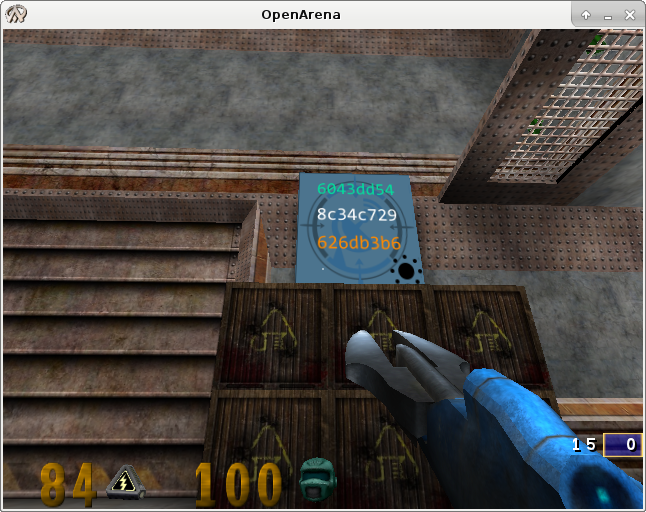
\includegraphics[width=9cm]{stage2/oashot-sun.png}
  \caption{Tuile hexadécimale dans la salle de départ}
  \label{shot2-sun}
\end{figure}

Un peu d'exploration de la carte révèle une grande salle avec des colonnes et des plateformes en hauteur avec des échelles pour y accéder, une autre petite pièce avec une grande cage au milieu, un couloir ``au sous-sol'' rempli d'eau qui contourne la seconde pièce.
L'exploration permet de trouver d'autres tuiles similaires à celle observée dans la salle de départ, ainsi que deux boutons.
Un bouton est situé au niveau des plateformes en hauteur de la grande salle et son activation a pour effet l'affichage d'un message ``15 seconds ...'' au centre de l'écran.
L'autre bouton est situé sur un mur de la pièce contenant la cage, son activation entraîne l'affichage du message ``The secret area is now open during 30 seconds !'' au centre de l'écran.
La ``zone secrète'' qui est ainsi ouverte correspond à un panneau derrière un gros logo SSTIC dans la grande salle, qui se lève pour révéler un troisième bouton pendant les 30 secondes suivant l'activation du second bouton (figure \ref{shot2-secretbutton}).

\begin{figure}[ht]
  \centering
  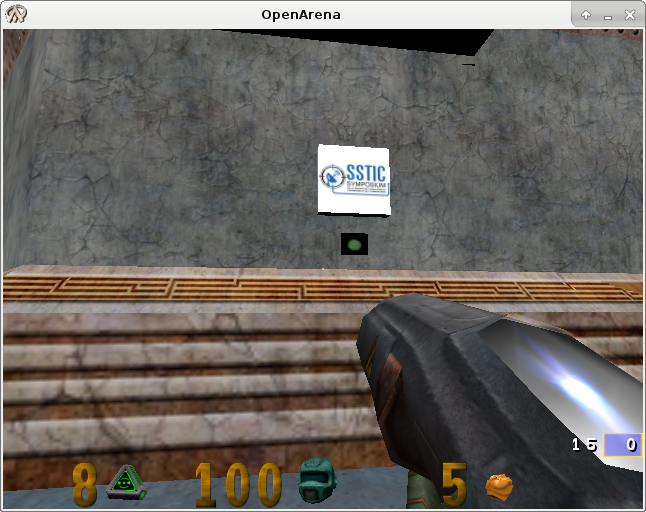
\includegraphics[width=9cm]{stage2/oashot-secretbutton.png}
  \caption{Troisième bouton dans la ``zone secrète''}
  \label{shot2-secretbutton}
\end{figure}

En tirant sur le troisième bouton, le joueur est téléporté dans une zone en dehors de la carte initiale, au milieu des étoiles, sur un chemin rectiligne traversé par des bassins de ce qu'il semble être de la lave.
Après avoir sauté au dessus de deux bassin, le joueur obtient un lance-roquette et le message ``Time to Rocket Jump ?!'' s'affiche à l'écran (figure \ref{shot2-rocketjump}).

\begin{figure}[ht]
  \centering
  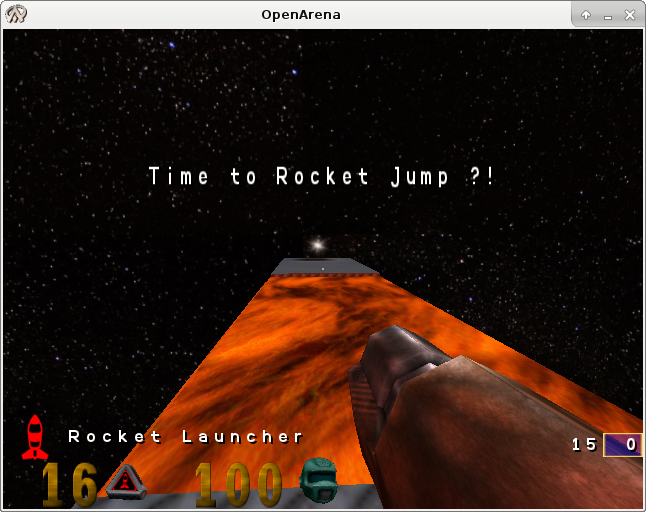
\includegraphics[width=9cm]{stage2/oashot-rocketjump.png}
  \caption{Le défi du saut roquette}
  \label{shot2-rocketjump}
\end{figure}

Le jeu semble indiquer qu'il faille utiliser un Trickjump\footnote{\url{https://en.wikipedia.org/wiki/Trickjump}} avec le lance-roquette\footnote{\url{http://www.trickingq3.com/Tutorials/Rocket_Tutorial.html}}.
Néanmoins ce saut est très difficile à réaliser et il ne faut pas oublier que ce jeu n'est qu'une étape d'un challenge de sécurité informatique (par opposition à un jeu réel).
Il est possible d'utiliser quelques codes de triche\footnote{\url{http://quake.wikia.com/wiki/Cheats_and_Console_Commands}} pour réussir le saut.

\clearpage
Par exemple:
\begin{itemize}
  \item \texttt{\bksl{}devmap sstic} permet de charger la carte avec les codes de triche activés,
  \item \texttt{\bksl{}god} permet d'être invincible et donc de ne pas mourir dans la lave,
  \item \texttt{\bksl{}noclip} permet de voler à travers la carte et de traverser les murs,
  \item \texttt{\bksl{}setviewpos -1900 610 -440 90} permet de se téléporter juste après le saut difficile.
\end{itemize}

Après le saut, le joueur trouve un quatrième bouton en hauteur.
Tirer dessus a pour effet d'être téléporté dans une salle qui contient sur le mur un assemblage de symboles et de couleurs (figure \ref{shot2-key}).

\begin{figure}[ht]
  \centering
  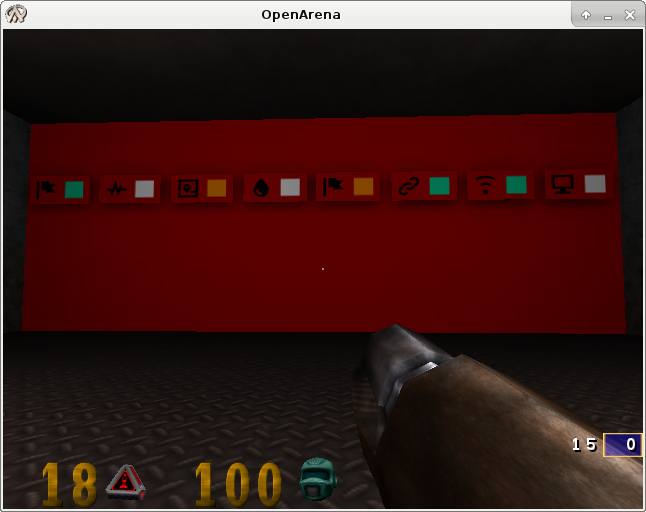
\includegraphics[width=9cm]{stage2/oashot-keywall.png}
  \caption{La clé de chiffrement dans le jeu}
  \label{shot2-key}
\end{figure}

Cela signifie certainement qu'il faut trouver dans la carte chaque tuile indiquée par les symboles et combiner les nombres hexadécimaux des couleurs correspondantes pour obtenir la clé.

\subsection{À la recherche des tuiles}

Voici où se trouve chaque tuile.

\begin{itemize}
  \item Dans la première pièce, sur les caisses\\
    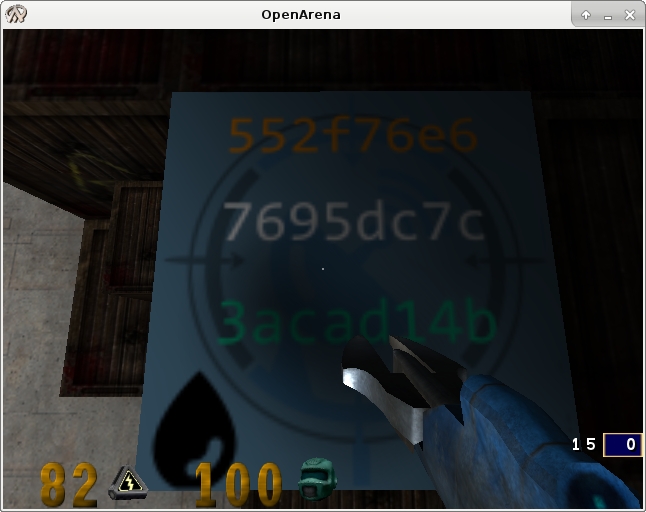
\includegraphics[width=7cm]{stage2/oashot-bead.png}
    \includegraphics[width=5cm]{stage2/bead-tile-out.png}
  \item Dans la grande salle, entre un bloc et un mur\\
    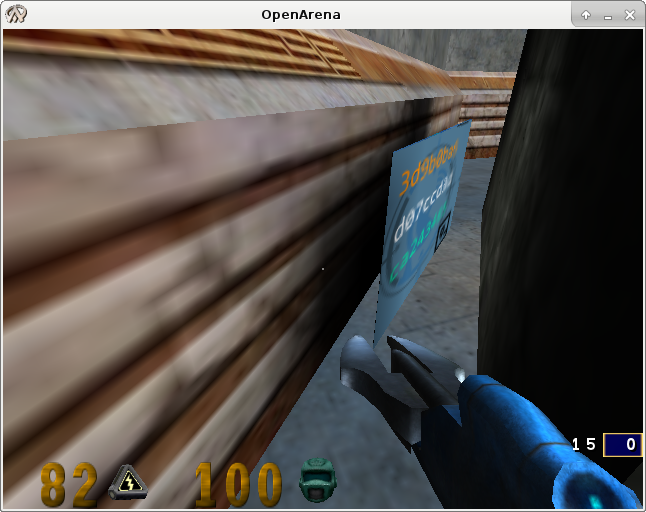
\includegraphics[width=7cm]{stage2/oashot-position.png}
    \includegraphics[width=5cm]{stage2/position-tile-out.png}
  \item Dans la grande salle, sur la plateforme mouvante\\
    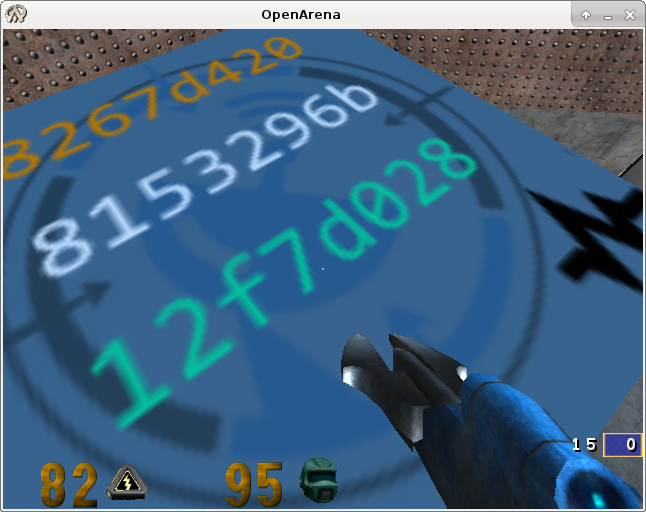
\includegraphics[width=7cm]{stage2/oashot-triangsig.png}
    \includegraphics[width=5cm]{stage2/triangsig-tile-out.png}
  \item Dans la petite pièce avec la cage, au dessus du bloc dans la cage\\
    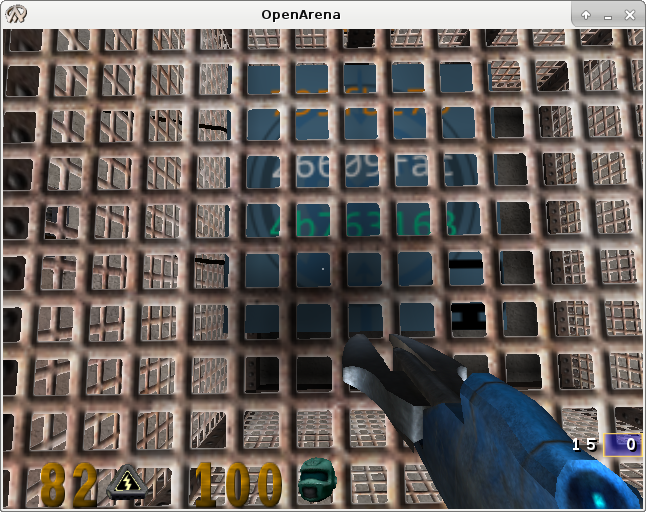
\includegraphics[width=7cm]{stage2/oashot-monitor.png}
    \includegraphics[width=5cm]{stage2/monitor-tile-out.png}
  \item Sous l'escalier qui mène au couloir rempli d'eau\\
    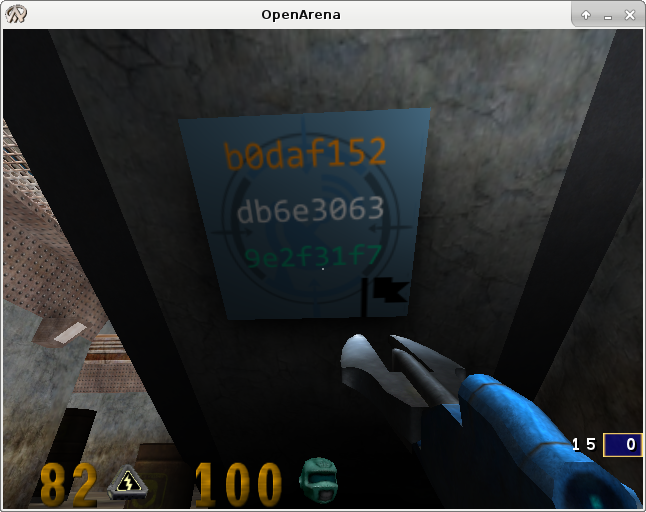
\includegraphics[width=7cm]{stage2/oashot-flag.png}
    \includegraphics[width=5cm]{stage2/flag-tile-out.png}
  \item Près de l'escalier, une fois le premier bouton activé\\
    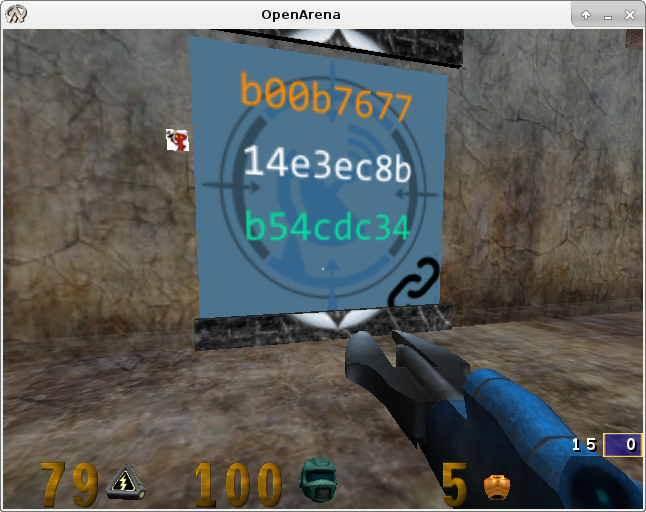
\includegraphics[width=7cm]{stage2/oashot-chain.png}
    \includegraphics[width=5cm]{stage2/chain-tile-out.png}
  \item Sur le trampoline à l'intersection entre plusieurs pièces\\
    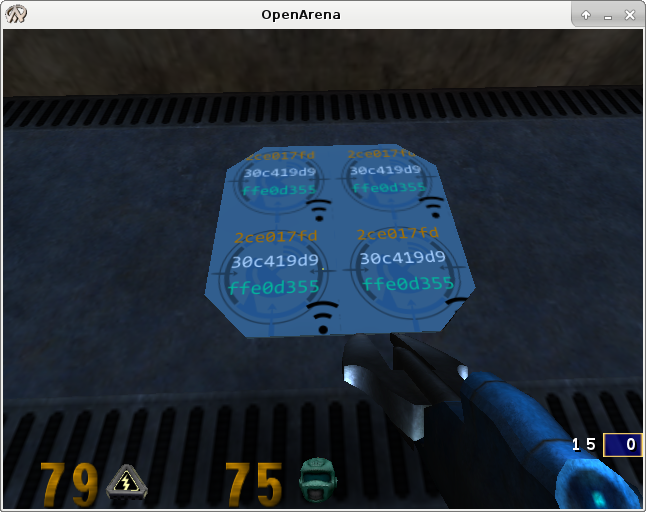
\includegraphics[width=7cm]{stage2/oashot-jump.png}
    \includegraphics[width=5cm]{stage2/jump-tile-out.png}
\end{itemize}

Ceci permet de décoder la clé:

\begin{tabular}{c c c c c c c c}
\includegraphics[width=1.45cm]{stage2/flag-green-out.png} &
\includegraphics[width=1.45cm]{stage2/triangsig-white-out.png} &
\includegraphics[width=1.45cm]{stage2/position-orange-out.png} &
\includegraphics[width=1.45cm]{stage2/bead-white-out.png} &
\includegraphics[width=1.45cm]{stage2/flag-orange-out.png} &
\includegraphics[width=1.45cm]{stage2/chain-green-out.png} &
\includegraphics[width=1.45cm]{stage2/jump-green-out.png} &
\includegraphics[width=1.45cm]{stage2/monitor-white-out.png} \\

\texttt{9e2f31f7} & \texttt{8153296b} & \texttt{3d9b0ba6} & \texttt{7695dc7c} &
\texttt{b0daf152} & \texttt{b54cdc34} & \texttt{ffe0d355} & \texttt{26609fac}
\end{tabular}

Finalement le fichier chiffré peut être déchiffré avec une commande \texttt{openssl}, en enlevant manuellement le padding.
\begin{verbatim}
% openssl enc -d -aes-256-ofb -in encrypted \
    -iv 5353544943323031352d537461676532 \
    -K 9e2f31f78153296b3d9b0ba67695dc7cb0daf152b54cdc34ffe0d35526609fac | \
  head -c -16 > decrypted

% sha256sum decrypted
845f8b000f70597cf55720350454f6f3af3420d8d038bb14ce74d6f4ac5b9187  decrypted

% file decrypted
decrypted: Zip archive data, at least v1.0 to extract
\end{verbatim}

La somme de contrôle du fichier déchiffré correspond bien à celle indiquée dans \texttt{memo.txt}, et ce fichier semble être une archive zip.
La partie suivante analyse le contenu de cette archive.

\clearpage
\section{Capture le Paint !}

La partie précédente a permis de déchiffrer un fichier en retrouvant la clé caché dans une carte OpenArena.
Le fichier déchiffré est une archive zip qui contient trois fichiers:
\begin{itemize}
  \item \texttt{encrypted}
  \item \texttt{memo.txt}
  \item \texttt{paint.cap}
\end{itemize}

Encore une fois, \texttt{memo.txt} contient des indications sur le contenu des deux autres fichiers:
\verbatiminput{stage3/memo.txt}

Ce fichier indique donc l'algorithme de chiffrement utilisé, le vecteur d'initialisation (qui est ``SSTIC2015-Stage3'' en hexadécimal) et deux sommes de contrôle, une pour le fichier chiffré (qui correspond bien au \texttt{encrypted} extrait de l'archive) et une pour le fichier déchiffré.

Pour comprendre ce que l'auteur de \texttt{memo.txt} entend par ``enregistrer de manière sécurisée avec Paint'', il faut analyser \texttt{paint.cap}.
La commande \texttt{file} indique qu'il s'agit d'une capture de paquets USB:
\begin{verbatim}
% file paint.cap
paint.cap: tcpdump capture file (little-endian) - version 2.4
(Memory-mapped Linux USB, capture length 262144)
\end{verbatim}

Un tel fichier peut être analysé avec Wireshark\footnote{\url{https://www.wireshark.org/}}.
Ceci permet de s'apercevoir que ce fichier contient:
\begin{itemize}
  \item 6 paquets dans lesquels l'hôte demande les descripteurs de périphérique à 3 clients et dans lesquels ceux-ci répondent, et en particulier le périphérique 3 annonce être une souris USB.
  \item Ensuite beaucoup de paquets dans lesquels le périphérique 3 envoie 4 octets et l'hôte accuse réception.
\end{itemize}

Les sources du noyau Linux permettent de comprendre la signification des 4 octets envoyés par la souris dans chaque paquet (fonction \texttt{usb\_mouse\_irq} de \texttt{drivers/hid/usbhid/usbmouse.c}\footnote{\url{http://git.kernel.org/cgit/linux/kernel/git/torvalds/linux.git/tree/drivers/hid/usbhid/usbmouse.c?id=v3.19\#n81}}):
\begin{itemize}
  \item le premier octet encode l'état des boutons (le bit de poids faible correspond au bouton gauche),
  \item le second encode le déplacement relatif selon la coordonnée X (de -128 à 127),
  \item le troisième encode le déplacement relatif selon la coordonnée Y (de -128 à 127), et
  \item le dernier encode le déplacement relatif selon la molette.
\end{itemize}

L'auteur a donc certainement enregistré les messages envoyés par sa souris pendant qu'il dessinait la clé de chiffrement dans Paint, ce qui explique son message dans \texttt{memo.txt}.

Pour reconstituer l'image dessinée, il suffit de suivre les mouvements de la souris en additionnant les déplacements relatifs, et de dessiner dans une image un point noir quand la souris se déplace avec le bouton gauche appuyé.

Voici un script Python qui utilise Scapy\footnote{\url{http://www.secdev.org/projects/scapy/}} pour décoder les paquets USB et Pillow\footnote{\url{http://python-pillow.github.io/}} pour dessiner. La figure \ref{fig-paint-out} présente le résultat obtenu.

\pyinput{stage3/decode_paint.py.inc.tex}

\begin{figure}[ht]
  \centering
  \includegraphics[width=10cm]{stage3/paint-out.png}
  \caption{Dessin reconstitué à partir de la capture des paquets USB}
  \label{fig-paint-out}
\end{figure}

Ainsi, la clé de chiffrement est le résultat de \texttt{BLAKE256("The quick brown fox jumps over the lobster dog")}.
La fonction BLAKE est un algorithme de hachage qui était finaliste dans le concours qui a déterminé SHA-3\footnote{\url{https://en.wikipedia.org/wiki/BLAKE_\%28hash_function\%29}} et même s'il n'est pas implémenté dans \texttt{openssl}, l'implémentation de référence est disponible sous licence CC0\footnote{\url{https://github.com/veorq/BLAKE}}.
Ceci permet de trouver la clé de chiffrement:
\begin{verbatim}
% printf 'The quick brown fox jumps over the lobster dog' | ./blake256 /dev/stdin
66c1ba5e8ca29a8ab6c105a9be9e75fe0ba07997a839ffeae9700b00b7269c8d /dev/stdin
\end{verbatim}

L'algorithme de chiffrement utilisé, Serpent, a été finaliste dans le concours qui a déterminé AES et n'est pas implémenté dans \texttt{openssl}.
Il faut donc écrire un programme court pour déchiffrer le fichier \texttt{encrypted}.
J'ai trouvé deux implémentations facilement utilisables de Serpent, l'une dans un module PHP\footnote{\url{http://php.net/manual/en/mcrypt.ciphers.php}}, l'autre dans la bibliothèque C++ Crypto++\footnote{\url{http://www.cryptopp.com/}}.
Comme je n'avais encore jamais écrit de programme avec Crypto++, j'ai utilisé cette bibliothèque dans la résolution du challenge.
Voici le programme C++ qui permet de déchiffrer \texttt{encrypted}.

\pyinput{stage3/decrypt.cpp.inc.tex}

J'ai compilé puis exécuté ce programme sur Linux avec les commandes suivantes:
\begin{verbatim}
% g++ -Wall -Wextra decrypt.cpp -o decrypt -lcryptopp -lpthread
% ./decrypt
\end{verbatim}

Ceci permet d'obtenir le fichier \texttt{decrypted} dont la somme de contrôle SHA-256 était dans \texttt{memo.txt}.
Il est donc possible de vérifier cette somme de contrôle et de se rendre compte que ce fichier est, encore une fois, une archive zip avec le contenu de l'étape suivante.
\begin{verbatim}
% sha256sum decrypted
7beabe40888fbbf3f8ff8f4ee826bb371c596dd0cebe0796d2dae9f9868dd2d2  decrypted

% file decrypted
decrypted: Zip archive data, at least v2.0 to extract
\end{verbatim}

\clearpage
\section{Cryptographie web}

\subsection{Décodage de Javascript obfusqué}

L'archive zip précédemment déchiffrée contient un seul fichier, nommé \texttt{stage4.html}.
Ce fichier commence par définir une feuille de style CSS puis contient entre les balises \texttt{<body>} et \texttt{</body>} trois lignes de Javascript particulièrement longues:
\begin{itemize}
  \item la première définit une variable \texttt{data} comme une chaîne de 528032 caractères hexadécimaux,
  \item la seconde est \texttt{var hash = "08c3be636f7dffd91971f65be4cec3c6d162cb1c";}, et
  \item la troisième contient du code Javascript sur 11580 caractères, sans aucun qui soit alphanumérique.
\end{itemize}

Les 5 premières instructions de la troisième ligne correspondent à du code Javascript obfusqué qui permet de construire des chaînes de caractères.
Voici ces instructions, avec des espaces et des commentaires pour mieux les comprendre.
\begin{verbatim}
$ = ~[];                    // $ = -1
$ = {
    ___: ++$,               // $.___ = 0
    $$$$: (![] + "")[$],    // $.$$$$ = "false"[0] = "f"
    __$: ++$,               // $.__$ = 1
    $_$_: (![] + "")[$],    // $.$_$_ = "a"
    _$_: ++$,               // $._$_ = 2
    $_$$: ({} + "")[$],     // $.$_$$ = "[object Object]"[2] = "b"
    $$_$: ($[$] + "")[$],   // $.$$_$ = ""undefined"[2] = "d"
    _$$: ++$,               // $._$$ = 3
    $$$_: (!"" + "")[$],    // $.$$$_ = "true"[3] = "e"
    $__: ++$,               // $.$__ = 4
    $_$: ++$,               // $.$_$ = 5
    $$__: ({} + "")[$],     // $.$$__ = "c"
    $$_: ++$,               // $.$$_ = 6
    $$$: ++$,               // $.$$$ = 7
    $___: ++$,              // $.$___ = 8
    $__$: ++$               // $.$__$ = 9
};
$.$_ = ($.$_ = $ + "")[$.$_$] +      // $.$_ = '[object Object]', add "c"
    ($._$ = $.$_[$.__$]) +           // $._$ = "o"
    ($.$$ = ($.$ + "")[$.__$]) +     // $.$$ = "n"
    ((!$) + "")[$._$$] +             // add "false"[3] = "s"
    ($.__ = $.$_[$.$$_]) +           // $.__ = "t"
    ($.$ = (!"" + "")[$.__$]) +      // $.$ = "r"
    ($._ = (!"" + "")[$._$_]) +      // $._ = "u"
    $.$_[$.$_$] + $.__ + $._$ + $.$; // add "ctor", $.$_ = "constructor"
$.$$ = $.$ + (!"" + "")[$._$$] + $.__ + $._ + $.$ + $.$$; // $.$$ = "return"
$.$ = ($.___)[$.$_][$.$_];           // $.$ = 0["constructor"]["constructor"]
\end{verbatim}

Après l'exécution de ces instructions, la variable \texttt{\$.\$\_} contient la chaîne de caractère \texttt{constructor} et \texttt{\$.\$\$} \texttt{return}.
Le contenu de \texttt{\$.\$} est plus complexe à comprendre.
Comme \texttt{0["constructor"]} renvoie la fonction interne \texttt{Number}\footnote{\url{http://www.w3schools.com/jsref/jsref_constructor_number.asp}}, \texttt{0["constructor"]} renvoie l'attribut \texttt{constructor} de \texttt{Number}, qui est la fonction interne \texttt{Function}.
Ainsi, \texttt{\$.\$} contient en quelque sorte un pointeur vers la fonction \texttt{Function}.

La sixième instruction, qui occupe le reste du code Javascript, est de la forme:
\begin{verbatim}
$.$($.$($.$$+"\""+ ... +"\"")())();
\end{verbatim}
... ce qui peut donc se décoder en:
\begin{verbatim}
Function( Function("return" + "\"" + ... + "\"")() )();
\end{verbatim}

La partie correspondant aux points de suspensions permet donc de construire un code Javascript qui sera renvoyé sous forme de chaîne de caractère par le premier appel à \texttt{Function}, puis exécuté juste après le second appel de \texttt{Function}.

Au passage, ces instructions correspondent exactement à celles qui sont décrites dans l'article \textit{Malware: Dollar Equals Tilde Square Brackets} du blog d'Avast\footnote{\url{https://blog.avast.com/2013/02/14/malware-dollar-equals-tilde-square-brackets/}}, datant de février 2013, mais cet article ne donne pas de détail sur la manière de décoder le code exécuté.

Pour effectuer ce décodage, j'ai commencé par isoler les trois lignes de code Javascript obfusqué dans un fichier à part, nommé \texttt{stage4.js}. Ensuite, j'ai créé un fichier \texttt{show\_jscode.html} dans le même dossier contenant:

\pyinput{stage4/show_jscode.html.inc.tex}

Le code Javascript de cette page HTML a pour effet d'appeler une fois la fonction \texttt{Function} pour obtenir une chaîne de caractère contenant le code Javascript décodé, et l'affiche tel quel.

Le code obtenu commence par \texttt{\_\_=document;\$\$\$='stage5';\$\$\_\$='load';} et définit ainsi un ensemble de variables nommées par des dollars et des soulignés.
Après la définition de ces variables, quatre fonctions sont définies.
La première ressemble à ceci (en ajoutant l'indentation):
\begin{verbatim}
function _____(______) {
    _ = [];
    for (___________ = _______; ___________ < ______[____________]; ++___________)
        _[____________________](______[___________________](___________));
    return new ______________________(_);
}
\end{verbatim}

Comme ce code est absolument illisible, il est nécessaire de renommer les variables constituées de soulignés par exemple par le nombre de soulignés qu'elles contiennent, préfixé par la lettre \texttt{v}.
Ceci peut être effectué automatiquement par cette commande shell:
\begin{verbatim}
% for i in $(seq 28 -1 3) ; do sed 's/_\{'$i'\}/v'$i'/g' -i decoded.js ; done
\end{verbatim}

Après cette transformation, la fonction précédente devient:
\begin{verbatim}
function v5(v6) {
    _ = [];
    for (v11 = v7; v11 < v6[v12]; ++v11)
        _[v20](v6[v19](v11));
    return new v22(_);
}
\end{verbatim}

En injectant également les définitions de variables précédentes, on obtient:
\begin{verbatim}
function v5(v6) {
    _ = [];
    for (v11 = 0; v11 < v6['length']; ++v11)
        _['push'](v6['charCodeAt'](v11));
    return new Uint8Array(_);
}
\end{verbatim}

Il s'agit donc d'une fonction permettant de transformer une chaîne de caractères en tableau d'entiers (de type \texttt{Uint8Array}) contenant les codes numériques de chaque caractère.
J'ai donc nommé cette fonction \texttt{str\_to\_u8arr} au cours de mon analyse.

En poursuivant le décodage du code en substituant les constantes là où elles sont utilisées, en transformant les accès aux attributs d'un object de \texttt{obj['attr']} en la notation équivalente \texttt{obj.attr}, en renommant quelques variables, et en ajoutant des commentaires, j'ai obtenu le code suivant.

\pyinput{stage4/decoded.js.inc.tex}

\clearpage

En résumé:
\begin{itemize}
  \item Ce script commence par afficher ``Download manager'' et ``loading...''.
  \item Il affiche également un lien caché vers \url{chrome://browser/content/preferences/preferences.xul}.
  \item Après une seconde, il exécute la fonction nommée avec 27 soulignés (nommée \texttt{v27} précédemment).
  \item Cette fonction détermine un vecteur d'initialisation et une clé de chiffrement en copiant respectivement les 16 premiers et les 16 derniers caractères de la première section entre parenthèses de l'agent utilisateur (obtenu par \texttt{window.navigator.userAgent}).
  \item Ensuite elle déchiffre le contenu de la variable \texttt{data} lue comme une chaîne de caractères hexadécimaux avec l'algorithme AES en mode CBC.
  \item La somme de contrôle SHA-1 du contenu déchiffré est comparée à la variable \texttt{hash}.
  \item Si la somme de contrôle correspond, le message ``loading...`` est remplacé par un lien de téléchargement portant le nom \texttt{stage5.zip}.
  \item Si une erreur est survenue précédemment, le message ``loading...`` est remplacé par le texte ``Failed to load stage5''.
\end{itemize}

\subsection{Déchiffrement}

Afin de déchiffrer le contenu de la variable \texttt{data}, il faut deviner le contenu à l'intérieur de la première parenthèse de l'agent utilisateur d'un navigateur particulier, ce qui permet d'obtenir le vecteur d'initialisation et la clé utilisée.

Pour cela, voici une liste d'hypothèses réalistes qu'il est possible d'établir:
\begin{itemize}
  \item Le navigateur utilisé est Firefox ou un de ses dérivés, car le lien caché \url{chrome://browser/content/preferences/preferences.xul} n'existe que dans ces types de navigateurs.
  \item Le système d'exploitation sur lequel le navigateur est installé est Windows, pour que le challenge soit cohérent avec la première étape, dans laquelle le script Rubber Ducky est spécifique à Windows.
  \item La version du navigateur utilisé est assez récente.
  \item Le fichier déchiffré est une archive zip, car le lien de téléchargement est nommé \texttt{stage5.zip}.
\end{itemize}

Ces hypothèses permettent de restreindre la recherche de l'agent utilisateur concerné aux versions de Firefox pour Windows situées entre les versions 29.0 et 37.0 (qui correspondent à la période de mi-2014 à avril 2015\footnote{\url{https://en.wikipedia.org/wiki/Firefox_release_history}}).

Un tel agent utilisateur ressemble à:
\begin{verbatim}
Mozilla/5.0 (Windows NT 6.3; rv:36.0) Gecko/20100101 Firefox/36.0
\end{verbatim}

Pour cet agent particulier, le vecteur d'initialisation (qui contient les 16 premiers caractères de ce qui est entre parenthèses) est ``\texttt{Windows NT 6.3; }'', et la clé (qui contient les 16 derniers caractères de la parenthèse) est ``\texttt{ NT 6.3; rv:36.0}''.

De rapides essais montrent que les quelques couples (vecteur d'initialisation, clé) que j'ai tentés sont mauvais.
Il faut donc élargir le bruteforce.
Mais avant cela, il est pertinent de remarquer que le mode CBC combiné au chiffrement d'une archive zip permet de tester les clés indépendamment du vecteur d'initialisation.
En effet, les données déchiffrées après le premier bloc (de 16 octets) ne dépendent pas du vecteur d'initialisation mais uniquement de la clé, comme indiqué par le schéma suivant.

\begin{figure}[ht]
  \centering
  
\includegraphics[width=14cm]{stage4/CBC-decryption.png}
  \caption{Mode d'opération CBC. Source: \url{https://en.wikipedia.org/wiki/Block_cipher_mode_of_operation\#CBC}}
  \label{fig-cbc-wikipedia}
\end{figure}

De plus, une archive zip est décodée à partir de la fin du fichier, et il est possible de vérifier la présence de la signature \texttt{PK} aux positions relatives -22 et -21 pour tester si une clé a une chance d'être correcte.

En prenant également en compte le rembourrage qui est ajouté au fichier clair avant chiffrement, le script suivant permet de tester un ensemble d'agents utilisateurs.

\pyinput{stage4/pseudo-brute.py.inc.tex}

Avec ce script, il s'avère qu'aucun agent utilisateur vérifiant les conditions établies ne fonctionne.
Par contre, en enlevant la contrainte du système d'exploitation, on obtient quasiment une archive zip (sans les 16 premiers octets) pour la clé ``\texttt{ X 10.6; rv:35.0}'', correspondant à Firefox 35.0 sur MacOS X 10.6.
Alors il devient très simple de deviner le reste du contenu de l'agent utilisateur, ``\texttt{Macintosh; Intel Mac OS X 10.6; rv:35.0}'', et donc le vecteur d'initialisation, \texttt{Macintosh; Intel}.

Pour obtenir le fichier zip déchiffré, il est possible de modifier le script Python pour enregistrer le contenu déchiffré, mais il est également possible d'utiliser le code obfusqué original (copié précédemment dans \texttt{stage4.js}) en modifiant l'agent utilisateur avant que le code soit exécuté.
Voici une page HTML qui effectue ceci.

\pyinput{stage4/show_downloadlink.html.inc.tex}

Cette page affiche un lien ``download stage5'' aussi bien avec Firefox que Chromium, sur Linux, et cliquer sur ce lien permet d'enregistrer un fichier nommé \texttt{stage5.zip}.

\clearpage
\section{Transputers}

\subsection{Découverte des transputers}
\label{sec5-1}

L'archive zip \texttt{stage5.zip} contient deux fichiers, nommés \texttt{input.bin} et \texttt{schematic.pdf}.
Le premier fichier est un fichier binaire d'un format inconnu avec quelques chaînes de caractères intéressantes (repérées en utilisant la commande \texttt{strings}):
\begin{itemize}
  \item les chaînes de caractères ``Boot ok'', ``Code Ok'' et ``Decrypt'', qui se succèdent de entre les positions 221 et 244 (en hexadécimal 0xdd à 0xf4)
  \item quatre caractères ``KEY\string:'' à la position 2437 (soit 0x985), et
  \item ``congratulations.tar.bz2'' à la position 2454 (soit 0x996).
\end{itemize}

Le second fichier est un document PDF d'une seul page dont le contenu est inclus dans la page suivante.
Ce document possède trois parties:
\begin{itemize}
  \item Un graphe de 14 rectangles bleus nommés \texttt{input.bin} et de \texttt{Transputer 0} à \texttt{Transputer 12}. Des nombres sont placés au début et à la fin de chaque ligne joignant les rectangles, sauf l'extrémité de la ligne connectant \texttt{input.bin}, qui est annotée \texttt{in/out}.
  \item Des sommes de contrôle SHA-256 pour deux fichiers, \texttt{encrypted} et \texttt{decrypted}, qui ne correspondent à aucun fichier extrait jusqu'à maintenant dans le challenge.
  \item Une section nommée ``Test vector'' qui contient du code Python 2 (reconnaissable à la structure \texttt{"\emph{nombre hexadécimal}".decode("hex")}) qui exécute une fonction \texttt{decrypt} appelée avec une clé et un bloc de données indiqués et compare le résultat obtenu avec la chaîne de caractères ``I love ST20 architecture''.
\end{itemize}

\clearpage
\includepdf{stage5/schematic.pdf}

Avant de chercher à savoir ce qu'est un transputer ou l'architecture ST20, il m'a semblé étrange que le document PDF mentionne un fichier \texttt{encrypted} sans que celui-ci soit présent dans l'archive \texttt{stage5.zip}.
En même temps, le fichier \texttt{input.bin} contient un nom de fichier, \texttt{congratulations.tar.bz2}, suivi par des octets qui semblent être inconnus mais qui pourraient correspondre au contenu chiffré de ce fichier.
Cette réflexion m'a amené à exécuter la commande suivante:
\begin{verbatim}
% dd if=input.bin bs=1 skip=2477 of=encrypted
250606+0 records in
250606+0 records out
250606 bytes (251 kB) copied, 0.886965 s, 283 kB/s

% sha256sum encrypted
a5790b4427bc13e4f4e9f524c684809ce96cd2f724e29d94dc999ec25e166a81  encrypted
\end{verbatim}

Ceci signifie que les 250606 octets à la position 2477 du fichier (juste après \texttt{congratulations.tar.bz2}) ont une somme de contrôle SHA-256 qui correspond exactement à celle indiquée pour le fichier \texttt{encrypted} dans le document PDF.
La probabilité d'une collision de somme de contrôle SHA-256 étant suffisamment faible pour être considérée nulle dans le cadre de ce challenge, il est possible d'affirmer que le fichier \texttt{encrypted} extrait de \texttt{input.bin} par la commande \texttt{dd} est précisément le fichier mentionné dans \texttt{schematic.pdf}.

Après avoir établi ceci, il reste à comprendre ce qu'est un transputer et ce à quoi correspond l'architecture ST20, à décoder la partie de \texttt{input.bin} qui précède le fichier chiffré, à trouver quel algorithme de déchiffrement il faut utiliser pour déchiffrer \texttt{encrypted}, et enfin trouver quelle clé utiliser (si elle n'est pas dans \texttt{input.bin}).

L'article Wikipedia consacré aux transputers\footnote{\url{https://en.wikipedia.org/wiki/Transputer}} permet de comprendre qu'il s'agit d'une architecture développée dans les années 1980 et que le ST20 est un microcontrôleur implémentant cette architecture.
Les transputers utilisent un jeu d'instruction de type RISC (Reduced Instruction Set Computing).
Peu d'outils actuels permettent de décoder ou d'exécuter un programme compilé pour l'architecture ST20, et encore moins permettent de comprendre le format utilisé pour \texttt{input.bin}.
Voici un rapide tour d'horizon qui est loin d'être exhaustif:
\begin{itemize}
  \item IDA supporte cette architecture \footnote{\url{https://www.hex-rays.com/products/ida/support/idadoc/618.shtml}} mais ne reconnaît pas le format de \texttt{input.bin}, et la version gratuite n'intègre pas de décompilateur, qui permettrait de comprendre plus rapidement les instructions.
  \item Quelques projets de décompilateur ST20 ne fournissent le code source, et le peu dont le code est gratuitement accessible sont peu lisibles (par exemple \url{https://github.com/Simo2553/AndroidPortings/tree/master/MonteDroid/Decompiler/Linux/frontend/machine/st20}).
  \item En ce qui concerne les émulateurs, il existe un projet ``ST20 emulator'' sur Sourgeforge\footnote{\url{http://sourceforge.net/projects/st20emu/}} dont le code est lisible rapidement, et permet au moins de comprendre l'organisation générale de l'architecture ST20.
  \item J'ai également trouvé un autre émulateur de transputer au code plutôt très lisible sur \url{http://spirit.lboro.ac.uk/emulator.html}.
  \item Ce site dispose d'un lien vers un projet plus récent dont l'auteur semble avoir utilisé une technique innovante pour publier son code source, en utilisant des fichiers PDF soit-disant sécurisés (\url{https://sites.google.com/site/transputeremulator/Home/source-code}).
\end{itemize}

En utilisant toutes les informations recueillies par diverses recherches sur internet ainsi qu'en lisant la documentation abondante disponibles sur \url{http://www.transputer.net/} (en particulier la liste des instructions\footnote{\url{http://www.transputer.net/iset/pdf/tis-sum.pdf}} et une annexe qui définit du vocabulaire utile\footnote{\url{http://www.transputer.net/iset/appendix/appendix.html}}), j'ai pu décoder le début du fichier \texttt{input.bin}.

\subsection{Code d'amorçage du transputer 0}

La lecture de la page Wikipedia anglaise sur les transputers permet de comprendre comment ceux-ci démarrent.
En effet, la section ``Booting''\footnote{\url{http://en.wikipedia.org/wiki/Transputer\#Booting}} indique qu'un transputer peut démarrer en téléchargeant un code d'amorçage sur le réseau.
Les données transmises pour cet amorçage consistent simplement en la taille du code, sur un octet, suivi du code proprement dit.
Comme sur le graphe des transputers de \texttt{schematic.pdf} le fichier \texttt{input.bin} est relié à la connexion 0 du transputer 0, il est raisonnable de penser que ce fichier commence par la séquence d'amorçage du premier transputer.
Le premier octet du fichier, f8 en hexadécimal, correspond donc a la taille du programme envoyé, soit 248 octets.

Voici les 249 premiers octets de \texttt{input.bin}.
\begin{verbatim}
% head -c 249 input.bin | xxd
00000000: f864 b440 d140 d324 f224 2050 23fc 64b4  .d.@.@.$.$ P#.d.
00000010: 2c49 21fb 24f2 48fb 2419 24f2 544c f724  ,I!.$.H.$.$.TL.$
00000020: 7921 a52c 4d21 fb24 f254 2479 f72c 4321  y!.,M!.$.T$y.,C!
00000030: fb24 7a24 79fb 6100 2419 24f2 514c fb24  .$z$y.a.$.$.QL.$
00000040: 1924 f252 4cfb 2419 24f2 534c fb29 4421  .$.RL.$.$.SL.)D!
00000050: fb24 f248 fb12 24f2 5444 f715 24f2 544c  .$.H..$.TD..$.TL
00000060: f728 4821 fb24 f248 fb13 24f2 5441 f719  .(H!.$.H..$.TA..
00000070: 24f2 5413 f1f7 40d4 1124 f254 41f7 1524  $.T...@..$.TA..$
00000080: f251 4cfb 1524 f252 4cfb 1524 f253 4cfb  .QL..$.RL..$.SL.
00000090: 1081 24f2 5541 f710 8224 f256 41f7 1083  ..$.UA...$.VA...
000000a0: 24f2 5741 f710 81f1 1082 f123 f310 83f1  $.WA.......#....
000000b0: 23f3 1081 23fb 11f1 7415 f2f1 742c f123  #...#...t...t,.#
000000c0: f310 23fb 1081 f174 15f2 23fb 7481 25fa  ..#....t..#.t.%.
000000d0: d4cc a380 40d4 1024 f241 fb66 0b42 6f6f  ....@..$.A.f.Boo
000000e0: 7420 6f6b 0043 6f64 6520 4f6b 0044 6563  t ok.Code Ok.Dec
000000f0: 7279 7074 0024 bc22 f0                   rypt.$.".
\end{verbatim}

Les données récupérées par le transputer 0 pour démarrer contiennent beaucoup de dollars et de lettres majuscules au début, et sont composées à la fin des trois chaînes de caractères qui ont été précédemment repérées dans \texttt{input.bin}.

Il faut donc maintenant décoder le programme qui est exécuté.
Pour cela, il est utile de donner quelques précisions sur l'architecture ST20 utilisée ici.
\begin{itemize}
  \item La mémoire utilisée est adressée sur 32 bits, et certaines instructions utilisent le concept de ``mot'' (``word'' en anglais), qui est un entier de 32 bits.
  \item Chaque instruction est codée sur 8 bits.
  \item Le système dispose de 6 registres de 32 bits, nommés \texttt{AReg}, \texttt{BReg}, \texttt{CReg}, \texttt{OReg}, \texttt{IPtr} et \texttt{WPtr}.
  \item Les trois premiers registres sont utilisés sous forme de pile. Les instructions qui chargent une valeur le font dans le registre \texttt{AReg} en déplaçant les valeurs de \texttt{AReg} et \texttt{BReg} respectivement dans \texttt{BReg} et \texttt{CReg}.
  \item Le registre \texttt{OReg} permet de construire les opérandes des instructions à l'aide des instructions \texttt{PFIX} et \texttt{NFIX}.
  \item Le registre \texttt{IPtr} est le pointeur d'instruction courante.
  \item Le registre \texttt{WPtr} est le ``Workspace Pointer'' (pointeur d'espace de travail). Il est souvent utilisé pour accéder à la mémoire du transputer.
\end{itemize}

Une instruction est un octet qui peut être lu sous la forme de deux chiffres hexadécimaux.
Le chiffre des unités est ajouté à \texttt{OReg} avant l'exécution de l'instruction et le second chiffre est utilisé pour déterminer l'instruction. Le jeu d'instruction de base contient donc 16 instructions, présentées dans le tableau ci-dessous avec chaque pseudo-code correspondant.
Dans le pseudo-code, \texttt{Push} signifie ``charger en haut de la pile'' et \texttt{Pop} ``décaler les valeurs de la pile vers le haut''.

\begin{tabular}{llll}
  \textbf{Mnémonique} & \textbf{Opcode} & \textbf{Signification} & \textbf{Pseudo-code} \\
  \texttt{J}     & \texttt{00} & Jump & \texttt{IPtr $\leftarrow$ IPtr + OReg} \\
  \texttt{LDLP}  & \texttt{00} & Load Local Pointer & \texttt{Push WPtr + 4 $\times$ OReg} \\
  \texttt{PFIX}  & \texttt{20} & Prefix & \texttt{OReg $\leftarrow$ OReg \lsl 4} \\
  \texttt{LDNL}  & \texttt{30} & Load Non-Local & \texttt{AReg $\leftarrow$ AReg[Oreg]} \\
  \texttt{LDC}   & \texttt{40} & Load Constant & \texttt{Push Oreg} \\
  \texttt{LDNLP} & \texttt{50} & Load Non-Local Pointer & \texttt{AReg $\leftarrow$ AReg + 4 $\times$ Oreg} \\
  \texttt{NFIX}  & \texttt{60} & Negative Prefix & \texttt{OReg $\leftarrow$ (\~{}OReg) \lsl 4} \\
  \texttt{LDL}   & \texttt{70} & Load Local & \texttt{Push WPtr[OReg]} \\
  \texttt{ADC}   & \texttt{80} & Add Constant & \texttt{AReg $\leftarrow$ AReg + Oreg} \\
  \texttt{CALL}  & \texttt{90} & Subroutine Call & \\
  \texttt{CJ}    & \texttt{a0} & Conditional Jump & \texttt{Si AReg = 0, IPtr $\leftarrow$ IPtr + OReg,} \\
                 &               &  & \texttt{sinon Pop} \\
  \texttt{AJW}   & \texttt{b0} & Adjust Workspace & \texttt{WPtr $\leftarrow$ WPtr + 4 $\times$ Oreg} \\
  \texttt{EQC}   & \texttt{c0} & Equals Constant & \texttt{AReg $\leftarrow$ (1 si AReg = Optr sinon 0)} \\
  \texttt{STL}   & \texttt{d0} & Store Local & \texttt{WPtr[Optr] $\leftarrow$ AReg, Pop} \\
  \texttt{STNL}  & \texttt{e0} & Store Non-Local & \texttt{AReg[Optr] $\leftarrow$ BReg, Pop, Pop} \\
  \texttt{OPR}   & \texttt{f0} & Operate & (dépend de la valeur de \texttt{OReg})
\end{tabular}

Après chaque instruction sauf \texttt{PFIX} et \texttt{NFIX} le registre \texttt{OReg} est réinitialisé à zéro.
Par ailleurs, pour les sauts, le registre \texttt{IPtr} est incrémenté avant l'exécution de l'instruction donc contient en pratique l'adresse de l'instruction suivante.
Les accès mémoires notés \texttt{WPtr[Optr]} et \texttt{AReg[Optr]} correspondent à des mots de 32 bits localisés respectivement aux adresses \texttt{WPtr} + 4 $\times$ \texttt{OReg} et \texttt{AReg} + 4 $\times$ \texttt{Oreg}.

L'instruction \texttt{CALL} sauvegarde l'état de la pile ainsi que \texttt{IPtr} dans \texttt{WPtr} avant de modifier \texttt{IPtr} pour matérialiser le saut, et l'instruction \texttt{OPR} permet d'exécuter une instruction étendue dont l'identifiant est dans \texttt{OReg}.

Le code exécuté par le transputer 0 commence par les octets \texttt{64 b4 40 d1} en hexadécimal, ce qui correspond donc aux instructions suivantes:

\begin{tabular}{lll}
  \textbf{Code hexadécimal} & \textbf{Instruction} & \textbf{Pseudo-code} \\
  \texttt{64} & \texttt{NFIX 4} & \texttt{OReg $\leftarrow$ (\~{}4) \lsl 4 = 0xffffffb0} \\
  \texttt{b4} & \texttt{AJW 4}  & \texttt{WPtr $\leftarrow$ WPtr + 4 $\times$ (0xffffffb0 + 4)} \\
  \texttt{40} & \texttt{LDC 0}  & \texttt{Push 0} \\
  \texttt{d1} & \texttt{STL 1}  & \texttt{WPtr[1] $\leftarrow$ AReg, Pop}
\end{tabular}

Les deux premières instructions peuvent être combinées en une unique instruction \texttt{AJW 0xffffffb4} pour faciliter la lecture.
De plus, le nombre hexadécimal de 32 bits ffffffb4 correspond au nombre -4c en utilisant la représentation du complément à 2, qui est pertinente ici car ce nombre est utilisé dans une addition, donc il est également possible d'utiliser la notation \texttt{AJW -0x4c} pour représenter l'instruction.

Les deux instructions suivantes on pour effet de charger la valeur 0 dans \texttt{WPtr[1]} (à l'adresse \texttt{WPtr + 4 $\times$ 1}, soit \texttt{WPtr + 4}).
Il est donc possible de les combiner dans le pseudo-code généré afin de faciliter la compréhension du code.

Après cette analyse, il est possible de décoder les 23 premiers octets du code du transputer 0.

\begin{tabular}{lll}
  \textbf{Code} & \textbf{Instruction} & \textbf{Pseudo-code} \\
  \texttt{64 b4} & \texttt{AJW -0x4c} & \texttt{WPtr $\leftarrow$ WPtr - 4 $\times$ 0x4c} \\
  \texttt{40 d1} & \texttt{LDC 0; STL 1}  & \texttt{WPtr[1] $\leftarrow$ 0} \\
  \texttt{40 d3} & \texttt{LDC 0; STL 3}  & \texttt{WPtr[3] $\leftarrow$ 0} \\
  \texttt{24 f2} & \texttt{OPR 0x42 (MINT)} & \texttt{Push 0x80000000} \\
  \texttt{24 20 50} & \texttt{LDNLP 0x400} & \texttt{AReg $\leftarrow$ AReg + 4 $\times$ 0x400} \\
  \texttt{23 fc} & \texttt{OPR 0x3c (GAJW)} & \texttt{WPtr $\leftrightarrow$ AReg} \\
  \texttt{64 b4} & \texttt{AJW -0x4c} & \texttt{WPtr $\leftarrow$ WPtr - 4 $\times$ 0x4c} \\
  \texttt{2c 49} & \texttt{LDC 0xc9} & \texttt{Push 0xc9} \\
  \texttt{21 fb} & \texttt{OPR 0x1b (LDPI)} & \texttt{AReg $\leftarrow$ AReg + IPtr} \\
  \texttt{24 f2} & \texttt{OPR 0x42 (MINT)} & \texttt{Push 0x80000000} \\
  \texttt{48}    & \texttt{LDC 8} & \texttt{Push 8} \\
  \texttt{fb}    & \texttt{OPR 0x0b (OUT)} & Envoie \texttt{AReg} octets depuis l'adresse \texttt{CReg} sur le canal \texttt{BReg}
\end{tabular}

Cette séquence d'instruction utilise quatre instructions étendues:
\begin{itemize}
  \item \texttt{MINT} (Minimum Integer) qui a pour effet de charger la valeur 0x80000000 dans la pile,
  \item \texttt{GAJW} (General Adjust Workspace), qui échange la valeur de \texttt{WPtr} avec le contenu du haut de la pile, \texttt{AReg},
  \item \texttt{LDPI} (Load Pointer to Insctruction), qui ajoute la valeur de \texttt{IPtr} à \texttt{AReg}, et
  \item \texttt{OUT} (Output), qui permet d'envoyer des données sur un lien.
\end{itemize}

Juste avant d'exécuter l'instruction \texttt{OUT}, trois valeurs sont poussées sur la pile:
\begin{itemize}
  \item La première valeur est la somme de 0xc9 et du pointeur d'instruction après l'instruction \texttt{LDPI}. Dans \texttt{input.bin}, ceci correspond donc à la position 0xc9 + 0x14 = 0xdd, qui correspond au début de la chaîne de caractères ``Boot ok''.
  \item La deuxième valeur est 0x80000000 et est interprétée comme un identifiant de canal. La lecture de documentation au sujet des transputers permet de comprendre que 0x80000000 correspond à l'écriture sur le lien 0, 0x80000004 à celle sur le lien 1, 0x80000008 sur le lien 2, etc.
  \item La troisième valeur est 8, qui est la longueur de ``Boot ok'' en prenant en compte le caractère terminateur (zéro ASCII).
\end{itemize}

Ainsi la première instruction \texttt{OUT} a pour effet d'envoyer la chaîne de caractères ``Boot ok'' sur le lien 0 du transputer 0.
Sur le schéma de \texttt{schematic.pdf} ce lien est annoté \texttt{in/out}.
On peut donc imaginer qu'il s'agit de la manière qu'ont les transputers pour transmettre des données ``ailleurs'' (par exemple dans un fichier, sur un moniteur, etc.), ce qui est communément appelé la \emph{sortie standard} par exemple dans les programmes C.

La suite de l'analyse du code du transputer 0 peut être réalisée à la main, mais j'ai préféré automatiser cette analyse en écrivant un décodeur qui affiche du pseudo-code au lieu des instructions réelles.
Cette approche a l'avantage de permettre ensuite une analyse très rapide des codes exécutés par les autres transputers.

Ainsi, j'ai écrit un script Python qui automatise cette analyse. Le code source du décodeur ST20 est disponible à l'annexe \ref{ann-5-decode-st20}, celui du script qui analyse le code du transputer 0 à l'annexe \ref{ann-5-decode-trans0}, et le pseudo-code généré à l'annexe \ref{ann-5-decode-trans0-out}.

Voici quelques indications permettant de comprendre le pseudo-code généré.
\begin{itemize}
  \item Tous les codes ont été décodés à partir de l'adresse 0. Ceci ne correspond pas à l'adresse réellement utilisée en mémoire (qui est nécessairement entre 0x8000000 et 0xffffffff selon les documents que j'ai trouvés), mais une rapide recherche ne m'a pas permis de déterminer quelle adresse était utilisée lors du démarrage de systèmes utilisant l'architecture ST20. Comme le code ne dépend pas fortement de là où il est chargé (grâce à l'instruction \texttt{LDPI} qui permet d'accéder aux données en utilisant un décalage relatif au pointeur d'instruction), le plus simple est de considérer que le code d'amorçage est chargé à l'adresse 0, ce qui ne change pas fondamentalement l'analyse.
  \item Les registres sont nommés \texttt{A}, \texttt{B}, \texttt{C} et \texttt{W} au lieu de \texttt{AReg}, \texttt{AReg}, \texttt{BReg}, \texttt{CReg} et \texttt{WPtr}.
  \item Au lieu d'utiliser la notation $A \leftarrow B$ pour les affectations j'ai utilisé $A = B$, mais le symbole égal dans ``\texttt{If A=0}'' correspond bien à un test d'égalité.
  \item L'instruction \texttt{IN}, qui permet de recevoir des données d'un lien, utilise la même convention d'appel que l'instruction \texttt{OUT}, avec la subtilité que les identifiants des canaux sont différents: 0x80000010 correspond au lien 0, 0x80000014 au lien 1, 0x80000018 au lien 2, etc.
  \item Les instructions \texttt{LB} (Load Byte) et \texttt{SB} (Store Byte), qui permettent respectivement de charger et d'enregistrer un octet dans une adresse donnée par \texttt{AReg} sont représentées en pseudo code par \texttt{LB(}adresse\texttt{)} et \texttt{SB:}adresse\texttt{ = }valeur. Ceci est lié au fait que la notation adresse\texttt{[}indice\texttt{]} a pour signification ``le nombre de 4 octets à l'adresse adresse + 4 $\times$ indice''.
\end{itemize}

\subsection{Décodage du code des transputers 0, 1, 2 et 3}

L'analyse du code du transputer 0 (en \ref{ann-5-decode-trans0-out}) montre que celui-ci est divisé en plusieurs parties:
\begin{itemize}
  \item La première partie, dont le code a été étudié manuellement à la section précédente, initialise quelques valeurs en mémoire puis envoie le message ``Boot ok'' sur le lien 0, qui correspond à la ``sortie standard'' du réseau de transputers.
  \item La deuxième, entre les adresse 17 et 35 en hexadécimal, consiste en une boucle dans laquelle le transputer reçoit 3 mots de 4 octets sur le lien 0 (connecté à \texttt{input.bin} dans \texttt{WPtr[0x49]}, \texttt{WPtr[0x4a]} et \texttt{WPtr[0x4b]} puis reçoit sur le lien 0 et retransmet \texttt{WPtr[0x49]} octets sur lien déterminé par l'identifiant dans \texttt{W[0x4a]}. Cette boucle est exécutée jusqu'à ce que \texttt{WPtr[0x49]} soit nul.
  \item Après la boucle le transputer envoie les 12 derniers octets reçus à chaque transputer qui lui est connecté (sur les liens 1, 2 et 3) et envoie ``Code Ok'' sur la sortie standard
  \item Il lit ensuite 4 octets dans \texttt{WPtr[2]} et 12 octets dans \texttt{WPtr[5]}, \texttt{WPtr[6]}\texttt{WPtr[7]} (ce qui sera noté \texttt{WPtr[5..7]} dans la suite) et envoie ``Decrypt'' sur la sortie standard.
  \item Il lit ensuite (dans le code à l'adresse 68) un octet dans \texttt{WPtr[3]} puis \texttt{WPtr[3]} octets dans \texttt{WPtr[9..]}.
  \item Après cela, le transputer entre dans une boucle infinie (entre les adresses 77 et db), qui sera décrite ensuite.
\end{itemize}

Cette analyse permet de comprendre l'organisation du fichier \texttt{input.bin}.
Après le code d'amorçage du transputer 0, celui-ci contient une succession de blocs de données que le transputer 0 transmet aux autres transputers, ces données étant formatées par un entête de 12 octets qui contient la longueur de la charge utile, sur 4 octets, et l'identifiant du lien sur lequel envoyer ces données, sur 4 octets.
Cette succession de blocs se termine par un bloc de taille nulle, qui se situe à la position 0x979 de \texttt{input.bin}.
Juste après (à la position 0x985) se trouvent quatre octets qui forment la chaîne de caractères ``KEY\string:'', suivi de 12 octets qui valent 0xff.
La mise en correspondance de ce contenu avec l'analyse du code du transputer 0 permet de comprendre que les 4 octets chargés dans \texttt{WPtr[2]} sont ceux de ``KEY\string:'' et les 12 chargés dans \texttt{WPtr[5..7]} sont ceux qui valent 0xff.
Après ceci se trouve un octet indiquant une longueur, qui vaut 23 (en décimal) puis la chaîne de caractères ``congratulations.tar.bz2'', qui occupe 23 octets.
Au moment d'arriver dans la boucle infinie, le prochain octet lu de \texttt{input.bin} par le transputer 0 correspond donc à l'octet à la position 0x9ad, qui est le premier octet de la partie correspond à ce qui a été précédemment identifié comme étant le fichier \texttt{encrypted}.

On peut ainsi en déduire que la boucle infinie du code du transputer 0 a pour but de déchiffrer le fichier \texttt{encrypted}, en utilisant les autres transputers pour exécuter l'algorithme de déchiffrement.

L'étape suivante dans l'analyse du réseau des transputers consiste donc à extraire le code d'amorçage des transputers 1, 2 et 3 à partir de \texttt{input.bin} et de l'analyser.
Comme les transputers 1, 2 et 3 suivent une procédure de démarrage similaire à celle du transputer 0, leurs codes d'amorçage correspond aux premiers blocs de données retransmis par le transputer 0 sur chacun des liens.
Il se trouve que les trois premiers blocs de données contiennent exactement le même contenu, mais adressé à chacun des liens.
Ainsi, il n'y a en pratique qu'un seul code à analyser.
Le script Python qui transforme le code extrait en pseudo-code est disponible à l'annexe \ref{ann-5-decode-trans123} et le pseudo-code résultant à l'annexe \ref{ann-5-decode-trans123-out}.

Ce code est très court et peut être étudié de manière similaire que pour le code du transputer 0:
\begin{itemize}
  \item Les transputers 1, 2 et 3 commencent par initialiser \texttt{WPtr}.
  \item Ensuite ils effectuent la même boucle que le transputer 0 pour relayer des blocs de données reçus par leur liens 0 et retransmis sur leurs autres liens, ce qui a pour effet d'initialiser les transputers 4 à 12.
  \item Par contre, il est important de noter que lorsqu'ils reçoivent un bloc de données dont l'entête annonce une longueur nulle, ce bloc n'est pas retransmis à tous les liens, contrairement à ce que fait le transputer 0. Ainsi le fait que le transputer 0 transmettre un tel bloc a pour effet de faire sortir les transputers 1 à 3 de leurs boucles de transmission de données, mais les transputers 4 à 12 utilisent certainement un code différent.
  \item Une fois la phase de ``relais de données'' terminée, une série d'instructions est exécutée en boucle, dans laquelle chaque transputer:
  \begin{itemize}
    \item reçoit 12 octets du lien 0 dans \texttt{WPtr[1..3]},
    \item retransmet ces 12 octets à chaque lien 1, 2 et 3,
    \item reçoit de chaque lien 1, 2 et 3 un octet,
    \item combine les 3 octets reçus par un ou exclusif bit-à-bit,
    \item envoi le résultat sur le lien 0.
  \end{itemize}
\end{itemize}

Les transputers 1, 2 et 3 agissent donc en temps qu'intermédiaires, tout d'abord pour initialiser le code des transputers 4 à 12, et ensuite pour combiner les opérations réalisées par ceux-ci.
La compréhension du code permet également de comprendre le mode de fonctionnement des opérations réalisées: 12 octets sont envoyés par le transputer 0 aux transputers 4 à 12 par l'intermédiaire de ceux 1 à 3, et le ``résultat'' consiste en un octet renvoyé au transputer 0 par l'intermédiaire des transputers 1 à 3, qui combinent les résultats intermédiaires par un ou exclusif bit-à-bit.

La reprise de l'analyse du code du transputer 0 (\ref{ann-5-decode-trans0-out}) permet de comprendre comment fonctionne la boucle qui effectue le déchiffrement (entre les adresses 77 et db):
\begin{itemize}
  \item Le transputer 0 commence une itération de la boucle en lisant dans \texttt{WPtr[1]} un octet provenant du lien 0 (dont de \texttt{input.bin}).
  \item Ensuite il envoie le contenu de \texttt{WPtr[5..7]} (qui fait 12 octets) sur les liens 1, 2 et 3, c'est-à-dire aux transputers 1, 2 et 3.
  \item Il reçoit un octet de chaque lien 1, 2 et 3 et les combine par ou exclusif binaire dans le second octet de \texttt{WPtr[0]} (à l'adresse \texttt{WPtr + 1}, ce qui est noté dans le pseudo-code par \texttt{SB:(ptr W[0])+1} et \texttt{LB((ptr W[0])+1)}).
  \item Puis il calcule dans le premier octet de \texttt{WPtr[0]} le résultat de \texttt{WPtr[1]\^{}(WPtr[4] + 2$\times x$)} où $x$ est l'octet à la position \texttt{WPtr[4]} dans \texttt{WPtr[5..7]}.
  \item Après ce calcul il met à jour l'octet à la position \texttt{WPtr[4]} dans \texttt{WPtr[5..7]} avec la valeur du second octet de \texttt{WPtr[0]}.
  \item Chaque itération de la boucle se termine par l'incrémentation modulo 12 de \texttt{WPtr[4]}, qui a au passage été initialisé à 0 juste avant la boucle, ainsi que par l'envoi du premier octet de \texttt{Wptr[0]} sur la sortie standard.
\end{itemize}

En résumé, \texttt{WPtr[5..7]} est un tableau de 12 octets dont un octet est modifié à chaque itération de la boucle par un octet déterminé en combinant les octets envoyés par les transputers 4 à 12 suite à l'envoi à ces transputers du contenu de \texttt{WPtr[5..7]}.
La valeur précédente de l'octet qui est ainsi mis à jour dans \texttt{WPtr[5..7]} est utilisé avec le compteur qui permet de repérer sa position pour déchiffrer à chaque itération un octet reçu sur le lien 0 et envoyer l'octet déchiffré de nouveau sur le lien 0.

L'algorithme de déchiffrement utilisé (qui par ailleurs a la propriété d'être identique à l'algorithme de chiffrement réciproque grâce au caractère involutif de la fonction utilisée pour calculer l'octet déchiffré) ne peut être étudié qu'après avoir extrait et décodé les codes utilisés par les transputers 4 à 12.
Pour cela, j'ai écrit un script Python (annexe \ref{ann-5-split-input}) qui lit \texttt{input.bin} et crée les fichiers contenant le code de chaque transputer, en affichant les positions du premier et dernier octet correspondant.
Le résultat affiché par ce script est disponible à l'annexe \ref{ann-5-split-input-out}.

\subsection{Transputers 4 à 12}

Chacun des transputers 4 à 12 commence par recevoir un programme d'amorçage qui est transmis par les transputers 1, 2 et 3.
Tous ces programmes d'amorçage sont identiques et sont relativement courts.
Une rapide analyse (effectuée par le script dont le code source est à l'annexe \ref{ann-5-decode-loader} et le pseudo-code généré à l'annexe \ref{ann-5-decode-loader-out}) permet de comprendre que ce programme:
\begin{itemize}
  \item reçoit sur le lien 0 trois entiers de 32-bits, enregistrés dans \texttt{WPtr[0]}, \texttt{WPtr[1]} et \texttt{WPtr[2]};
  \item reçoit \texttt{WPtr[0]} octets sur le lien 0, enregistrés à partir de la position 0x1f relative par rapport à l'adresse de la première instruction du programme d'amorçage;
  \item exécute le code nouvellement téléchargé en plaçant la position 0x1f + \texttt{WPtr[2]} dans \texttt{IPtr}.
\end{itemize}

L'entête de trois entiers qui précède le code réellement exécuté contient donc la longueur de ce code ainsi que la position de la première instruction à exécutée, qui en pratique est toujours \texttt{0xc} (cf. \ref{ann-5-split-input-out}).

Il est donc maintenant possible d'extraire le code exécuté sur chacun des transputers 4 à 12 et de l'analyser pour reconstruire l'algorithme de déchiffrement qui a été implémenté.
Pour cela, j'ai écrit un script Python dont le code est situé à l'annexe \ref{ann-5-decode-main} et le pseudo-code extrait à l'annexe \ref{ann-5-decode-main-out}.

L'exécution de chaque code commence à l'adresse 0xc, après la définition de deux fonctions que j'ai nommées \texttt{recv(chan=B, mem=C, len=W[0])} et \texttt{send(chan=B, mem=C, len=W[0])} et qui concrètement utilisent les instructions \texttt{IN} et \texttt{OUT} pour recevoir ou envoyer des données.

La lecture et la compréhension des pseudo-codes permet alors d'écrire en C une fonction qui déchiffre \texttt{size} octets contenus à l'emplacement \texttt{src} dans un bloc mémoire alloué en \texttt{dst} en utilisant la clé \texttt{key}:

\pyinput{stage5/decrypt-transputers.c.inc.tex}

Comme il est très facile de faire des erreurs lors de l'écriture de ce code C, il est utile d'avoir un moyen réaliste de tester l'implémentation.
Heureusement, le fichier \texttt{schematic.pdf} contient un \emph{Test vector} permettant de réaliser un tel test: le déchiffrement des données indiquées avec la clé ``*SSTIC-2015*'' devrait produire le texte ``I love ST20 architecture'', ce qui est le cas.

L'étude des transputers a ainsi permis de déterminer l'algorithme de déchiffrement utilisé et de le réimplémenter en C.
L'analyse des transputers est donc maintenant terminer et l'étape suivante consiste maintenant à trouver la clé permettant de déchiffrer le fichier chiffré.

\subsection{Attaque par force brute de la clé}

Dans le code du transputer 0, la clé de 12 octets utilisée pour le déchiffrement des données est initialisée en lisant 12 octets de valeur 0xff dans \texttt{input.bin}.
Néanmoins cette clé ne permet pas de déchiffrer correctement le fichier chiffré extrait à la section \ref{sec5-1} (la somme de contrôle SHA-256 est donnée dans \texttt{schematic.pdf}).
Il faut donc trouver la clé à utiliser.

Pour cela, voici les informations qui ont été recueillies précédemment.
\begin{itemize}
  \item Le fichier déchiffré s'appelle probablement \texttt{congratulations.tar.bz2} et est donc une archive compressée avec le format BZip2.
  \item Le fichier déchiffré fait la même taille que le fichier chiffré, 250606 octets.
  \item Dans l'algorithme de déchiffrement, la clé de déchiffrement est utilisée quasiment directement pour déchiffrer les 12 premiers octets, son contenu n'ayant pas été modifié par les transputers.
\end{itemize}

L'article Wikipedia consacré à BZip2 permet d'apprendre que l'entête d'un fichier dans ce format contient presque toujours les même 10 premiers octets, qui sont en hexadécimal \texttt{42 5a 68 39 31 41 59 26 53 59}.
De plus, comme le fichier est relativement petit, il est possible de supposer que le champ \texttt{origPtr} de l'entête est inférieur à $2^{17}$, ce qui signifie, en supposant également que le champ \texttt{randomised} est nul, que l'octet à la position 14 (en décimal) est probablement nul.
Cette hypothèse est discutable mais permet toutefois de considérablement accélérer le bruteforce de la clé de déchiffrement et donc de se rendre compte relativement rapidement si elle est juste ou fausse.

Pour les 12 premiers octets, le déchiffrement des données consiste à effectuer cette opération pour tout $i$ entre 0 et 11 (l'opérateur \^{} correspondant au ou exclusif bit-à-bit sur 8 bits et \emph{mod} à l'opération modulo):
\begin{displaymath}
  \mbox{déchiffré}[i] \leftarrow \mbox{chiffré}[i] \mbox{ \^{} } ((i + 2 \times \mbox{clé}[i]) \mod 256)
\end{displaymath}

Comme déchiffré$[i]$ et chiffré$[i]$ sont connus pour $i$ entre 0 et 9 (grâce à l'entête BZip2), il est possible de vérifier que déchiffré$[i]$ \^{} chiffré$[i] - i$ est pair et ensuite d'en déduire que pour tout $i$ entre 0 et 9,
\begin{displaymath}
  \mbox{clé}[i] \mod 128 = \frac{(\mbox{déchiffré}[i] \mbox{ \^{} } \mbox{chiffré}[i] - i) \mod 256}{2}
\end{displaymath}

Cette équation donne donc directement les 7 bits de poids faible des 10 premiers octets de la clé.
Il reste à trouver le bit fort de chacun de ces 10 octets ainsi que les deux derniers octets de la clé, c'est-à-dire au total $10 + 2 \times 8 = 26$ bits.
Pour tester de manière automatique si chaque possibilité est valide, il est possible de comparer la somme de contrôle SHA-256 des données déchiffrées à la somme de contrôle indiquée dans \texttt{schematic.pdf}.
Au moment du challenge je n'ai pas utilisé cette méthode car dans les étapes précédentes, la présence d'un rembourrage à la fin des données déchiffrées a fait qu'il est arrivé que la somme de contrôle fournie ne corresponde pas directement au résultat déchiffré (il fallait enlever le rembourrage).
À la place, j'ai utilisé la bibliothèque bzlib pour tenter de décompresser les données déchiffrées, en sachant que le format BZip2 contient une somme de contrôle CRC32 des données décompressées, qui assure l'intégrité du fichier.
Ceci est certes légèrement plus complexe mais en pratique a mené au bon résultat.

Par ailleurs, l'hypothèse qui a été faite que l'octet à la position 14 soit nul permet d'interrompre rapidement le déchiffrement des données après 3 itérations de la boucle de déchiffrement.
En effet, après 3 itérations, la clé contient à la position 2 la valeur qui sera utilisée ensuite pour déchiffrer l'octet à la position 14 et il est donc possible de déchiffrer spécifiquement cet octet sans attendre 12 autres itérations.

Cette astuce permet de trouver en 12 minutes 24 secondes la clé de déchiffrement en utilisant un seul thread sur un processeur Intel Core i7 cadencé à 2,2 GHz.
Le code utilisé pour réaliser le bruteforce est présenté à l'annexe \ref{ann-5-brute}.

La clé de déchiffrement trouvée est alors, en hexadécimal:
\begin{verbatim}
5e d4 9b 71 56 fc e4 7d e9 76 da c5
\end{verbatim}

Ceci permet de finalement déchiffrer le fichier \texttt{encrypted} puis de vérifier que la somme de contrôle SHA-256 du fichier obtenu correspond bien à celle attendue dans \texttt{schematic.pdf}:
\begin{verbatim}
% sha256sum congratulations.tar.bz2
9128135129d2be652809f5a1d337211affad91ed5827474bf9bd7e285ecef321  congratulations.tar.bz2
\end{verbatim}

\clearpage
\section{Quelques derniers petits efforts en image}

\subsection{Une première image}

L'archive \texttt{congratulations.tar.bz2} déchiffrée par le réseau de transputers contient un unique fichier nommé \texttt{congratulations.jpg}, qui est une image JPEG contenant le message ``Félicitations... un dernier petit effort ?'', avec le logo du SSTIC et des diablotins qui ont déjà été rencontrés précédemment dans la carte OpenArena.

\begin{figure}[ht]
  \centering
  \includegraphics[width=9cm]{stage6/congratulations.jpg}
  \caption{\texttt{congratulations.jpg}}
  \label{fig6-jpg}
\end{figure}

L'utilisation de \texttt{binwalk} permet de trouver rapidement la suite du challenge, qui a été simplement concaténée à l'image.
Voici les commandes que j'ai effectuées avec ce qu'elles affichent dans le terminal.
\begin{verbatim}
% binwalk congratulations.jpg

DECIMAL       HEXADECIMAL     DESCRIPTION
--------------------------------------------------------------------------------
0             0x0             JPEG image data, JFIF standard  1.01
55248         0xD7D0          bzip2 compressed data, block size = 900k

% dd if=congratulations.jpg of=hidden1.tar.bz2 bs=1 skip=55248
197321+0 records in
197321+0 records out
197321 bytes (197 kB) copied, 0.728172 s, 271 kB/s

% tar tjf hidden1.tar.bz2
congratulations.png
\end{verbatim}

\subsection{Une deuxième image}

L'archive au format tar.bz2 cachée dans l'image \texttt{congratulations.jpg} contient un unique fichier, nommé \texttt{congratulations.png}, qui contient le message ``Félicitations... deux derniers petit efforts ?'' (figure \ref{fig6-png}).

\begin{figure}[ht]
  \centering
  \includegraphics[width=9cm]{stage6/congratulations.png}
  \caption{\texttt{congratulations.png}}
  \label{fig6-png}
\end{figure}

Une analyse avec Wireshark de l'image révèle la présence de blocs du type non-standard \texttt{sTic} au sein de l'image PNG (capture d'écran en figure \ref{fig6-shot-pngwireshark}).
Il semble donc pertinent d'extraire ces blocs afin d'en étudier le contenu.
Il apparaît alors que le contenu extrait a été compressé avec la bibliothèque zlib.

\begin{figure}[ht]
  \centering
  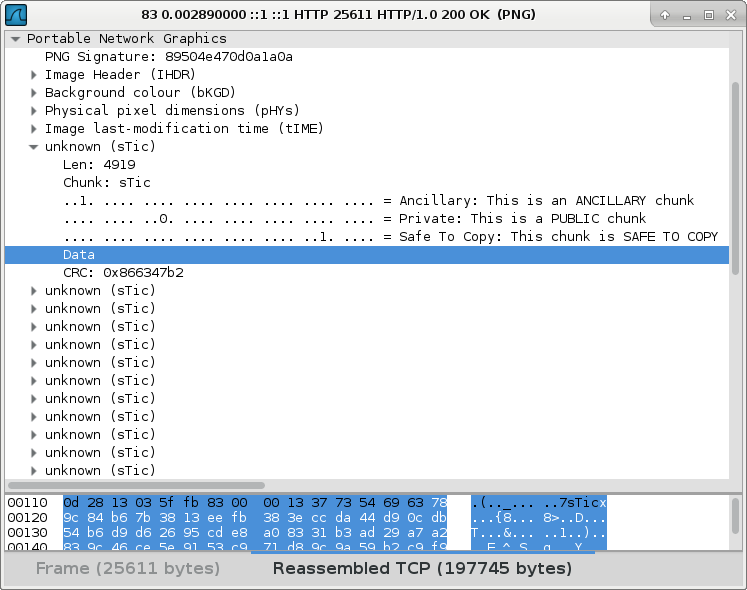
\includegraphics[width=16cm]{stage6/shot-pngwireshark.png}
  \caption{Analyse dans Wireshark de \texttt{congratulations.png}}
  \label{fig6-shot-pngwireshark}
\end{figure}

\clearpage

Voici le script Python que j'ai utilisé pour extraire et décompresser les blocs de données de l'image.

\pyinput{stage6/extract2_from_png.py.inc.tex}

Ceci permet d'obtenir une nouvelle archive, au format tar.bz2.

\subsection{Jamais deux sans trois}

La troisième archive contient une image nommée \texttt{congratulations.tiff} similaire aux précédentes, et cette fois au format TIFF.
En la comparant pixel à pixel avec les images précédentes, il apparait que l'image est quasiment identique à la première (\texttt{congratulations.jpg}, au texte près).
Plus précisément, dans la moitié supérieure de chaque image, une grande partie des pixels ont le bit de poids faible des composantes rouge et verte qui diffèrent entre les deux images, le reste des bits étant toujours égaux.
Ceci indique probablement qu'un algorithme de stéganographie a été utilisé pour cacher des données dans les bits de poids faible des composantes rouge et verte de certains pixels de l'image TIFF.

En combinant ces bits, il est possible d'arriver à une archive tar.bz2 valide.
Voici un script Python qui extrait cette archive de l'image:

\pyinput{stage6/extract3_from_tiff.py.inc.tex}

\subsection{La dernière image}

Une quatrième fois, l'archive obtenue contient une image de félicitations, \texttt{congratulations.gif}.
Cette image GIF utilise une palette de 256 couleurs qui contient beaucoup de cases de couleur noire sans raison logique apparente.

\begin{figure}[ht]
  \centering
  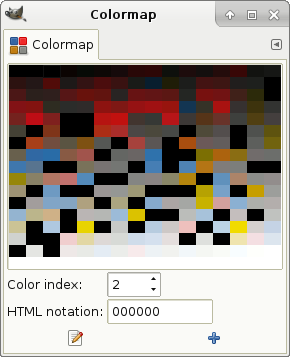
\includegraphics[width=5cm]{stage6/shot-gifcolormap.png}
  \caption{Palette des couleurs de \texttt{congratulations.gif} dans GIMP}
  \label{fig6-gifcolormap}
\end{figure}

En modifiant la couleur d'indice 2 de la palette (initialement noir), on se rend compte que cet indice est utilisé par les pixels du cadre noir de l'image, sauf certains qui forment une adresse e-mail.
Il s'agit de l'adresse e-mail qu'il faut trouver pour résoudre le challenge, et l'image GIF est donc l'image qui marque la fin du challenge.

\begin{figure}[ht]
  \centering
  \includegraphics[width=10cm]{stage6/solution.png}
  \caption{Remplacement de la couleur 2 par une couleur de notation HTML b5e6ff dans \texttt{congratulations.gif}}
  \label{fig6-solution}
\end{figure}

\clearpage
\section{Conclusion}

Le challenge 2015 du SSTIC est constitué de six étapes très différentes les unes des autres.
Les résoudre toutes nécessite de mettre en œuvre des compétences variées: décodage de format peu répandu (pour le script Rubber Ducky, la capture des mouvements de souris...), compréhension d'un jeu d'instruction ancien mais documenté (pour les transputers), résolution d'une énigme dans une carte OpenArena, recherche d'astuces pour accélérer une attaque par force brute, etc.
Ce document a présenté comment j'ai résolu ce challenge, en détaillant les divers outils que j'ai utilisés et les déductions logiques que j'ai réalisées.

Tous les programmes utilisés pour résoudre le challenge sont des logiciels libres.
L'ensemble du code que j'ai écrit pour le challenge (scripts Python et programmes C/C++) ainsi que les fichiers ayant servis à générer ce document \LaTeX{} seront disponibles à l'adresse \url{https://github.com/fishilico/sstic-2015} une fois le challenge terminé.
Tout ceci est publié sous la licence Beerware\footnote{\url{https://en.wikipedia.org/wiki/Beerware}}\footnote{\url{https://tldrlegal.com/license/beerware-license}}.

\section{Remerciements}

Je souhaite tout d'abord remercier les concepteurs du challenge, qui ont conçu un challenge intéressant même si le scénario est très linéaire.
J'ai apprécié découvrir OpenArena et le monde des transputers, ainsi que l'API Javascript permettant d'utiliser des routines de chiffrement dans un navigateur.

Je souhaite ensuite remercier ceux qui ont organisé le challenge du premier avril, qui a l'avantage d'être une entrée en matière simple pour des personnes qui s'intéressent à l'informatique au sens large et à qui j'ai pu donner un rapide aperçu des concepts fondamentaux de la résolution des challenges SSTIC, à savoir l'utilisation d'outils modernes pour résoudre des énigmes difficiles.

Je remercie ensuite tout ceux qui m'ont permis de participer au challenge en me permettant d'avoir un cadre de vie adapté à Singapour, où je vis depuis quelques mois, ainsi que tous ceux qui m'ont motivé malgré le fait que je participais ``pour le plaisir, uniquement sur mon temps libre et quand je n'avais rien de plus important à faire, comme aller me balader en Malaisie (ce que j'ai fait le jour de la sortie du challenge) ou participer aux célébrations de Pâques (ce que j'ai fait le lendemain)''.

\clearpage
\begin{appendices}
\section{Scripts utilisés}

Cette section regroupe les divers scripts que j'ai écrits pour la résolution du challenge et qui n'ont pas été mis dans les parties précédentes.

\subsection{Partie 1, décodeur des invocations PowerShell}
\label{ann-1-powerdecode}

\pyinput{stage1/powerdecode.py.inc.tex}

\subsection{Partie 5, extraction des parties du fichier \texttt{input.bin}}
\label{ann-5-split-input}

\pyinput{stage5/split_input.py.inc.tex}

\subsection{Partie 5, décodeur des instructions ST20}

\subsubsection{Générateur de pseudo-code ST20}
\label{ann-5-decode-st20}

Ce fichier s'appelle \texttt{decode\_st20.py}

\pyinput{stage5/decode_st20.py.inc.tex}

\subsubsection{Décodeur du code du transputer 0}
\label{ann-5-decode-trans0}

\pyinput{stage5/decode_trans0.py.inc.tex}

\subsubsection{Décodeur du code des transputers 1, 2 et 3}
\label{ann-5-decode-trans123}

\pyinput{stage5/decode_trans123.py.inc.tex}

\subsubsection{Décodeur du code d'amorçage des transputers 4 à 12}
\label{ann-5-decode-loader}

\pyinput{stage5/decode_loader.py.inc.tex}

\subsubsection{Décodeur du code principal des transputers 4 à 12}
\label{ann-5-decode-main}

\pyinput{stage5/decode_all_main.py.inc.tex}

\subsubsection{Attaque par force brute de la clé de déchiffrement}
\label{ann-5-brute}

\pyinput{stage5/decrypt.c.inc.tex}

\clearpage
\section{Sortie produite par les scripts de la partie 5}

\subsection{Organisation du fichier \texttt{input.bin}}
\label{ann-5-split-input-out}

Voici la sortie du script dont le code a été donné dans la partie \ref{ann-5-split-input} et qui présente l'organisation du contenu du fichier \texttt{input.bin}.

\verbatiminput{stage5/input-desc-out.txt}

\subsection{Pseudo-code généré par l'analyse des codes des transputers}

Voici la sortie des scripts de la partie \ref{ann-5-decode-st20}.

\subsubsection{Pseudo-code du transputer 0}
\label{ann-5-decode-trans0-out}

\verbatiminput{stage5/code-trans0-out.txt}

\subsubsection{Pseudo-code des transputers 1, 2 et 3}
\label{ann-5-decode-trans123-out}

\verbatiminput{stage5/code-trans123-out.txt}

\subsubsection{Pseudo-code d'amorçage des transputers 4 à 12}
\label{ann-5-decode-loader-out}

\verbatiminput{stage5/code-loader-out.txt}

\subsubsection{Pseudo-code principal des transputers 4 à 12}
\label{ann-5-decode-main-out}

\verbatiminput{stage5/code-all-main-out.txt}

\end{appendices}

\end{document}
